\documentclass[11pt,letterpaper]{article}

\usepackage[T1]{fontenc}
\usepackage{lmodern}
\usepackage{microtype}
\usepackage[margin=1in]{geometry}
\linespread{1.0}
\setlength{\parskip}{0pt}
\setlength{\parindent}{1.5em}

\usepackage{amsmath,amssymb,amsthm}
\usepackage{graphicx}
\usepackage{xcolor}
\usepackage{tikz}
\usetikzlibrary{arrows.meta,positioning}
\usepackage{booktabs,tabularx,array,longtable}
\newcolumntype{L}[1]{>{\raggedright\arraybackslash}p{#1}}
\newcolumntype{Y}{>{\raggedright\arraybackslash}X}
\usepackage{listings}
\usepackage{upquote}
\lstset{basicstyle=\ttfamily\footnotesize,breaklines=true,columns=fullflexible,frame=single,framesep=4pt,showstringspaces=false,captionpos=b}
\usepackage[hidelinks]{hyperref}
\usepackage{cleveref}

\usepackage{everypage}
\definecolor{grokgray}{RGB}{110,110,110}
\AddEverypageHook{%
  \ifnum\value{page}=1
    \begin{tikzpicture}[remember picture, overlay]
      \node[rotate=90, anchor=south, font=\footnotesize\sffamily\color{grokgray}, inner sep=0pt]
        at ([xshift=30pt, yshift=0.5\paperheight]current page.south west)
        {GrokRxiv:2026.10.partitioned-derived-data\quad [\,cs.DC\,]\quad 20 Oct 2026};
    \end{tikzpicture}
  \fi
}

\newtheorem{theorem}{Theorem}[section]
\newtheorem{proposition}[theorem]{Proposition}
\newtheorem{lemma}[theorem]{Lemma}
\newtheorem{corollary}[theorem]{Corollary}
\theoremstyle{definition}
\newtheorem{definition}[theorem]{Definition}
\newtheorem{assumption}[theorem]{Assumption}
\theoremstyle{remark}
\newtheorem{remark}[theorem]{Remark}

\newcommand{\id}{\mathrm{id}}
\newcommand{\tree}{\tau}
\newcommand{\R}{\mathsf{R}}
\newcommand{\W}{\mathsf{W}}
\newcommand{\Pfx}{\mathcal{P}}
\newcommand{\Keys}{\mathcal{K}}
\newcommand{\Ch}{\mathrm{Ch}}
\newcommand{\Eval}{\mathrm{Eval}}
\newcommand{\dom}{\mathrm{dom}}
\DeclareRobustCommand{\code}[1]{{\def\_{\textunderscore\allowbreak}\texttt{#1}}}

\title{Partitioned Derived Data\\[4pt]
  {\normalsize Part II of \emph{Source Code as a Transactional Abstraction}}}
\author{Matthew Long\\
  \small The YonedaAI Collaboration, YonedaAI Research Collective\\
  \small Chicago, IL\\
  \small \texttt{matthew@yonedaai.com} $\cdot$ \texttt{https://yonedaai.com}}
\date{October 2026}

\begin{document}
\maketitle

\begin{abstract}
Source code and source control can now be treated as transactional abstractions: a repository is a database, a change is a transaction with a read set and a write set, and a version is a snapshot. This paper supplies the part of that foundation that concerns derived data. We model search indexes, symbol tables, blame and work plans as views over the transaction log, maintained incrementally by partitioned jobs over immutable snapshots in the manner of Spark's resilient distributed datasets, and stated over abstract primitives: an object store, a durable queue and stateless compute. We prove that a maintained view is consistent at a snapshot, equal to full recomputation, whenever the key under which each partition result is stored determines that result, a condition we call key sufficiency, and that the work per commit is then proportional to the size of the changed partitions. Content addressing subsumes recursion from parent commits and shares results across branches, while history-dependent views such as blame need the commit id as key. In the reference implementation, YonedaRepo on Cloudflare, the search key is a bare subtree id and is not sufficient, so a renamed or duplicated directory receives a view that names the wrong paths. An executed test confirms this view-consistency failure, and we give two repairs. A partitioned codemod is serializable under backward validation only if it declares its directory scope as a read. Indexing cost was not measured; the evidence is tests, including asserted rebuild counts of 3, 1 and 0.
\end{abstract}

\section{Introduction}
\label{sec:pdd:intro}

Source code and source control are now transactional abstractions. The series this paper belongs to treats a repository as a database: a change is a transaction with a read set and a write set, landing a change is a commit under optimistic concurrency, and a version is a snapshot \cite{long2026partI}. Derived data complete the picture. A search index, a symbol table or a blame is a view of a snapshot, and it must stay consistent with the snapshot it claims to describe while many transactions land. This Part lays that piece of the foundation: a definition of derived data as views over the transaction log maintained incrementally by partitioned jobs, the condition under which incremental maintenance is correct at a snapshot, and a working realization in which one view violates the condition.

We argue that the next evolution in code is transactional, and the argument rests on precedent. Data lakes began as files on object stores. Concurrent writers and derived computation broke file-level semantics, and the field moved to tables with a transaction log, snapshots and optimistic concurrency \cite{armbrust2020delta}, over which Spark-style partitioned computation runs \cite{zaharia2012rdd}. Source control is under the same pressure, because agents multiply both the number of concurrent writers and the volume of derived work, and for code the derived work, from search and symbols to checks and the Git objects themselves, becomes views over the log. Scion's published design makes the same move: changesets are entries in a log, created separately from ref updates, and a ref moves by compare-and-set on one database row \cite{anthropic2026scion}. The proofs and measurements of this series support the thesis; they do not settle it.

A repository holds two kinds of data. Inherent data are the commits, trees and blobs that users write. Derived data are everything computed from them: the trigram index that answers code search, the table of symbols in each file, the attribution of each line to the commit that last changed it, the history of a path, the review class of a change, the result of a check on a commit. A repository with one human committer can recompute most derived data on demand. A repository that lands tens of thousands of changes per day cannot. The Scion post reports more than 30,000 merges per day at Anthropic in September 2026 \cite{anthropic2026scion} % S-2
and describes derived data as values defined recursively over a changeset's parents and computed by one generic mechanism \cite{anthropic2026scion}. Mononoke, the server of Meta's Sapling, implements the same idea through a trait whose central method derives a value for one changeset from its Bonsai representation and its parents' derived values \cite{mononokederived}.

The question this paper answers is when such reuse is correct and what it costs. The answer has to be precise because the failure mode is silent. A stale or misattributed index returns plausible results. An incremental build that reuses the wrong partition produces a search hit at a path that does not exist, or a codemod that skips a file, and nothing in the request reports an error.

Part~I treats the repository as a Delta-style table: an append-only transaction log, snapshots identified by log versions, and optimistic concurrency with backward validation \cite{armbrust2020delta}. This Part treats derived data as Spark-style partitioned jobs over those snapshots \cite{zaharia2012rdd}. A job names a snapshot commit, a partitioning of its tree, a task kind and a policy. Map tasks read immutable objects through the object tiers and write one segment per partition. A reduce combines segments into the answer. Write jobs, such as a repository-wide literal replacement, reduce instead into a single commit that enters the transaction log through Part~I's validation.

The architecture is stated over cloud-portable primitives, and YonedaRepo, the system under study, is its reference realization on Cloudflare. The author designed and built YonedaRepo, which is still being built; its code is cited by file and commit throughout and in Appendix~\ref{app:pdd:evidence}.

Its derived-data layer partitions a commit's root tree by top-level directory, keys each directory's segment by the directory's Git tree id, and stores segments in the object store under that key. The design notes describe the goal as ``only changed partitions recompute''. A test confirms the behavior on a three-partition repository: the first query builds three segments, a query after a change to one directory builds one, and a query pinned at the earlier log version builds none (Section~\ref{sec:pdd:evidence}).

We make six contributions.
\begin{enumerate}
\item A job model and a formal definition of content-local and history-dependent derivation kinds over the commit DAG (Sections~\ref{sec:pdd:jobs} and~\ref{sec:pdd:fold}).
\item A view-consistency theorem: partition reuse equals full recomputation exactly when the storage key is sufficient for the map function, with a work bound proportional to the changed partitions and a soundness result for pruning by the log's touched paths (Section~\ref{sec:pdd:incremental}).
\item A view-consistency failure in the reference implementation. The search segment key omits the directory prefix, while the segment records full paths, so the key is not sufficient and the maintained view can disagree with its snapshot. We give two repairs and prove both correct (Section~\ref{sec:pdd:prefix}).
\item An analysis of write jobs. A codemod is atomic, and it is serializable with concurrent landings only if it is confined to a directory that it declares as a read, or if it lands as a fast-forward (Section~\ref{sec:pdd:write}).
\item Properties of the symbol-level plan DAG, including the exact sense in which Tarjan components and stages realize the companion paper's independence condition and critical-path bound \cite{long2026inversion}, and the condition under which the planner inherits the companion paper's representation invariance (Section~\ref{sec:pdd:plan}).
\item Git compatibility as a derived view: the Git commits of main are a deterministic projection of the log, rebuilt incrementally, with a measured staleness (Section~\ref{sec:pdd:git}).
\end{enumerate}

The evidence for correctness is tests, and the evidence for cost is almost absent. The tests are the repository's unit and property-based tests and a test we wrote against the code at commit \code{cfa4845} that executes the counterexample of Section~\ref{sec:pdd:prefix}. The only timings that touch derived data are the commit-time derivation phase in two instrumented hosted runs and the warm-start seed figures from commit messages. Indexing throughput, segment sizes, the fraction of partitions that change on real repositories and the cost of a codemod were not measured; Part~III, Section~9 lists the planned measurements \cite{long2026partIII}.

\section{Setting and imported objects}
\label{sec:pdd:setting}

The object store holds Git blobs, trees and commits addressed by their Git object ids (Part~I, Definition~4.1). A commit $c$ has an ordered list of parents, the first of which is $\pi_1(c)$. Its tree state $\tree(c)$ maps file paths to blob ids and modes; the commit's root tree encodes it. For a path prefix $p$ we write $\tree(c)|_p$ for the subtree at $p$ when it exists, and $\id(\tree(c)|_p)$ for the id of the Git tree object that encodes it. The platform records with each commit its touched paths, a list that contains every path whose entry differs between $\tree(\pi_1(c))$ and $\tree(c)$ (Part~I, Definition~4.2). The transaction log $(e_1,\ldots,e_n)$ of a repository (Part~I, Definition~4.10) records, for each version $v$, the ref it moved, the old and new commit, and the touched paths $\W_v$ of the commit it appended (Part~I, Definition~4.8). A snapshot $S_v$ is the ref map after version $v$ (Part~I, Definition~4.11), and a read pinned at version $v$ or at a commit id sees an immutable tree (Part~I, Definition~4.13).

Concurrency control works on accesses. Accesses are file paths, directory prefixes written \code{dir/}, or symbol entries \code{path\#symbol}, with an overlap relation $\bowtie$ (Part~I, Definition~4.4). Each change has a declared read set $\R$ and a write set $\W$, which the platform may refine to symbols (Part~I, Definition~4.6), and two work items are independent in the sense of the companion paper's \cite[Eq.~1]{long2026inversion} condition when neither writes what the other reads or writes (Part~I, Definition~4.7). Landing a change validates it backward against the entries that landed after its base version, with outcomes fast-forward, rebase, merge or conflict (Part~I, Definition~4.15).

The proofs of Sections~\ref{sec:pdd:write} and~\ref{sec:pdd:vacuum} rest on four results of Part~I, which we use in the following form.
\begin{description}
\item[\normalfont (P1)] Validation of a change with base $b$ and declared reads $\R$ returns a conflict if some later entry on the same ref is opaque or has a refined write that overlaps $\R$; otherwise it returns fast-forward, rebase or merge, and in the last two cases the platform appends a merge commit whose parents are the previous head and the landed commit (Part~I, Definition~4.15).
\item[\normalfont (P2)] If validation does not return a conflict, the tree after landing equals the tree before landing with the change's writes applied, and the declared reads agree between the base and the state just before landing (Part~I, Theorem~6.4).
\item[\normalfont (P3)] The land combiner validates each batch member against the log but not against the other members, so a batch can contain two members that each write what the other read (Part~I, Theorem~7.3); if the combiner also refuses a member whose reads overlap the writes of an earlier accepted member, the batch is equivalent to landing its members one at a time in ticket order (Part~I, Proposition~7.4).
\item[\normalfont (P4)] If a ref holds commit $x$ at version $u$, then at every later version its value reaches $x$ by first parents (Part~I, Theorem~5.4).
\end{description}

One property of Git objects carries most of the arguments below. A tree object lists names, modes and object ids of its entries, and its own id is the hash of that listing \cite{gitobjects}. Trees therefore form a Merkle structure \cite{merkle1988}.

\begin{assumption}[Collision resistance]
\label{as:pdd:collision}
Over all objects a repository ever stores, distinct object contents have distinct ids. The same holds for the platform digest $H$ over the values it is applied to, each of which is encoded unambiguously before hashing. Part~I makes the same assumption for object ids in all its results (Part~I, Section~4).
\end{assumption}

\begin{lemma}[Subtree identity]
\label{lem:pdd:merkle}
Under Assumption~\ref{as:pdd:collision}, two stored trees have the same id if and only if they have the same entries recursively: the same names, the same modes and the same file contents at every path. In particular, for commits $c,c'$ and a prefix $p$, $\id(\tree(c)|_p)=\id(\tree(c')|_p)$ if and only if every file below $p$ has the same mode and content in both commits.
\end{lemma}

\begin{proof}
If the ids are equal, Assumption~\ref{as:pdd:collision} gives equal tree contents, so the entry lists are equal. Equal entry lists contain equal child ids, and induction on depth gives equal subtrees and blobs at every path. Conversely, Git serializes a tree with its entries in a canonical order determined by name and mode, so recursively equal trees serialize to the same bytes and hash to the same id \cite{gitobjects}.
\end{proof}

The lemma is the reason a tree id can stand for the content of a whole directory. It says nothing about where the directory sits. Two directories with different names and identical content have the same id, and this fact is the source of the defect analyzed in Section~\ref{sec:pdd:prefix}.

\begin{lemma}[Commit ids determine ancestry]
\label{lem:pdd:ancestry}
Under Assumption~\ref{as:pdd:collision}, the id of a commit determines its root tree, its parent ids in order, and recursively the root trees and parents of all its ancestors.
\end{lemma}

\begin{proof}
A commit object contains its tree id and its parent ids \cite{gitobjects}. Equal commit ids give equal commit objects, hence equal tree and parent ids; induction along parents gives the rest.
\end{proof}

The job model needs four primitives besides Part~I's serialized authority, which holds the log. An \emph{object store} holds segments under keys, with puts and gets. A \emph{durable queue} delivers derivation jobs at least once, with retries. \emph{Stateless compute} runs map and reduce tasks as request handlers. \emph{Container compute} runs checks. The results of this Part are stated over these primitives and use only the properties just listed, plus the read guarantee of Assumption~\ref{as:pdd:store}. The reference realization uses Cloudflare R2, Queues, Workers and Containers, and Part~III, Table~1 maps each primitive to its realizations \cite{long2026partIII}.

Some limits of the reference realization bind derived data, and each comes from one realization's choice, not from the design. Each Worker invocation, the stateless-compute primitive here, allows six simultaneous outgoing connections and a fixed subrequest budget \cite{cfworkerslimits}, which bounds how many partitions one invocation can build at once. R2, the object store here, allows one concurrent write per second to a key \cite{cfr2limits}, which matters only when two jobs write the same key. Another realization would change these numbers and leave the theorems untouched. Part~III, Section~4 treats the limits in full.

\section{The job model}
\label{sec:pdd:jobs}

\begin{definition}[Partitioning]
\label{def:pdd:partitioning}
Let $c$ be a commit whose root tree has directory entries $d_1,\ldots,d_r$ and non-directory entries $F$. The partitioning of $c$ is the set
\[
\Pi(c)=\{(d_i,\tree(c)|_{d_i}) : 1\le i\le r\}\cup\{(\varepsilon,F)\},
\]
where the last term is omitted when $F$ is empty. Its canonical order lists the directory partitions in tree-entry order and the root-files partition last, as the implementation emits them. Its elements are pairs of a prefix and the object that the partition covers. The first kind of partition covers every file below one top-level directory. The second, the root-files partition, covers the files directly in the root. A key function $\kappa$ assigns each partition a storage key.
\end{definition}

The implemented key function sets $\kappa(d,x)=\id(x)$ for a directory partition and $\kappa(\varepsilon,F)=\text{\code{files-}}\,\|\,H(\lambda(F))$ for the root-files partition, where $\lambda(F)$ is the text listing each root file's name and blob id and $H$ is the platform digest (\code{plan} in \path{platform_derived.rs}). Every file path has a unique first component, so the partitions of a commit are pairwise disjoint in the paths they cover and together cover every file. The root listing omits file modes. That suffices for search and symbol extraction, whose map functions do not read modes; a mode-dependent kind would need modes in $\lambda(F)$. This disjointness is what lets a write job take the union of per-partition changes without conflict between partitions (Section~\ref{sec:pdd:write}).

\begin{definition}[Derivation kind]
\label{def:pdd:kind}
A content-local derivation kind is a triple $\delta=(S_\delta,f_\delta,\rho_\delta)$. The map function $f_\delta$ sends a partition $(p,x)$ to a segment in $S_\delta$. The reduce function $\rho_\delta$ sends a finite family of prefixed segments, in the canonical order of Definition~\ref{def:pdd:partitioning}, to a value. The full value of $\delta$ at commit $c$ is
\[
D_\delta(c)=\rho_\delta\bigl(\langle (p,\,f_\delta(p,x)) \rangle_{(p,x)\in\Pi(c)}\bigr).
\]
A kind is history-dependent when its value at $c$ is not a function of $\tree(c)$ alone.
\end{definition}

We call $D_\delta(c)$ the \emph{view} of kind $\delta$ at the snapshot pinned at commit $c$. A system maintains the view incrementally when it answers from stored partial results instead of recomputing $D_\delta(c)$, and the maintained view is \emph{consistent at the snapshot} when its answer equals $D_\delta(c)$. Every correctness statement in this Part is a statement of view consistency. The terms follow the materialized-view literature, in which a materialized view behaves like a cache of a query's result and incremental maintenance rests on the observation that only part of a view changes after an update \cite[Section~1]{gupta1995maintenance}.

Code search is the main content-local kind. Its map function builds a segment for a partition: the list of files with their full paths, blob ids and an \emph{indexed} flag, together with a posting list from each case-folded trigram to the files containing it (\code{build\_segment} in \path{search.rs}). Files larger than 1~MiB or detected as binary are listed but not indexed. Its reduce answers a query by intersecting postings in each segment, reading candidate blobs, matching lines and concatenating the per-partition results up to a limit.

\begin{definition}[Job]
\label{def:pdd:job}
A job is a tuple $J=(c,\Pi,\delta,\mathit{pol})$ of a snapshot commit, a partitioning, a derivation kind and a policy. The policy carries the caller's grant, the limits that apply to the job and, for checks, the digest of the repository's landing policy. A read job returns $D_\delta(c)$ or a query answer computed from it. A write job returns a single commit whose parent is $c$ (Definition~\ref{def:pdd:writejob}).
\end{definition}

\begin{definition}[Segment store and evaluator]
\label{def:pdd:segment-store}
A segment store is a partial map $\Sigma:\Keys\rightharpoonup S_\delta$ with operations $\mathrm{get}(k)$ and $\mathrm{put}(k,s)$, where a put overwrites. The incremental evaluator $\Eval_\Sigma(c)$ computes, for every $(p,x)\in\Pi(c)$, the key $k=\kappa(p,x)$; if $k\in\dom\Sigma$ it uses $\mathrm{get}(k)$, and otherwise it computes $s=f_\delta(p,x)$, performs $\mathrm{put}(k,s)$ and uses $s$. It then applies $\rho_\delta$ to the family of prefixed segments.
\end{definition}

Definition~\ref{def:pdd:segment-store} is a direct transcription of \code{searchSegments} in \path{repo-derived.ts}. The function asks the Rust \code{search\_plan} operation for the partitions of the root tree, looks up each key at \path{derived/v1/<repo>/search/<key>} in R2, builds missing segments with the Rust \code{index\_partition} operation and writes them back. All partitions are processed concurrently with \code{Promise.all} inside one Worker invocation, and the function returns the number of segments it built. A partition with more than 20,000 files is not indexed; the evaluator reports it as too large, and the search response lists it under \code{skipped\_partitions}.

The Rust operations never fetch objects themselves. They return \code{need\_trees} or \code{need\_blobs}, the adapter fetches the named objects through the tiered object reader and calls again, for at most 257 rounds (\code{withObjects} in \path{repo-derived.ts}). Each supplied blob is checked against its id before use (\code{verified\_blob} in \path{platform_derived.rs}), which is Part~I's object-verification invariant~I5 applied to derived data (Part~I, Table~3). A map task's input is therefore exactly the content its key names, even when the adapter is not trusted.

Jobs run at two times. A landing that moves a ref enqueues on the durable queue a message naming the repository and the ref. In the reference implementation the message has kind \code{platform\_derive} (\path{repo-tools.ts}), and the consumer, a Cloudflare Queue configured with batch size 1 and three retries, reads the ref's current head and builds its search segments and a warm-start seed for check runs (\code{deriveAfterLanding} in \path{repo-derived.ts}). A query that finds a segment missing builds it on demand. Because the message names the ref and not the commit, a burst of landings produces messages that each derive whatever head is current when they run. Later messages find their segments already built and do no map work. This coalescing is correct by Theorem~\ref{thm:pdd:incremental}, since a job duplicated by at-least-once delivery, or delayed, computes values that are already in the store or that the store would hold anyway.

\begin{table}[t]
\centering
\small
\caption{The Spark analogy made concrete. The left column follows the resilient distributed datasets paper \cite{zaharia2012rdd} and the companion paper's mapping \cite{long2026inversion}; the right column names the implemented counterpart.}
\label{tab:pdd:spark}
\begin{tabularx}{\textwidth}{@{}L{3.2cm}YY@{}}
\toprule
Spark concept & Counterpart in YonedaRepo & Difference \\
\midrule
Partition of a dataset & A top-level subtree of a commit, or the root files & Partitions are fixed by repository layout, not chosen by the planner \\
Narrow transformation & A map task that builds one segment from one subtree & The task is a pure function of verified objects \\
Lineage & The key of a segment, which names the subtree it was built from & Lineage is a content hash, not a chain of operators \\
Persistence & Segments stored in the object store under their keys & Segments persist across commits and branches and are never evicted by the platform \\
Recovery after loss & Rebuilding a missing segment from immutable objects & Recomputation is exact because inputs never change \\
Shuffle & The reduce of a write job into one commit, and cross-partition symbol references & The only cross-partition coordination is the commit and its validation \\
Stage & A stage of the plan DAG over agent work items & The platform plans stages but does not execute agent work \\
Scheduler & One stateless-compute invocation running all partitions concurrently & Partitions are not yet fanned out through the durable queue \\
\bottomrule
\end{tabularx}
\end{table}

Table~\ref{tab:pdd:spark} records the analogy and where it bends. The bend that matters most for capacity is the last row. The design fans partition tasks out through the durable queue and workflow primitive. The reference implementation runs every partition of a job in one Worker invocation, so a job's parallelism there is bounded by that invocation's six simultaneous connections and its subrequest budget \cite{cfworkerslimits}; a fan-out realization on any platform would remove that bound. The analogy holds for the data model and the recovery argument. It does not yet hold for distributed execution.

\section{Derived data as a fold over the commit DAG}
\label{sec:pdd:fold}

The Scion post and Mononoke define derived data recursively from parents. Content addressing defines it from the tree. The two definitions agree for content-local kinds, and the difference between them is what content addressing can reuse.

\begin{definition}[Parent-recursive derivation]
\label{def:pdd:fold}
A parent-recursive derivation of kind $\delta$ is a function $\Phi_\delta$ such that for every commit $c$ with parents $c_1,\ldots,c_r$,
\[
D_\delta(c)=\Phi_\delta\bigl(c,\;D_\delta(c_1),\ldots,D_\delta(c_r)\bigr),
\]
with $D_\delta(c)=\Phi_\delta(c)$ for a root commit. Evaluating $D_\delta$ at every commit in topological order is a fold over the commit DAG.
\end{definition}

Mononoke's \code{derive\_single} has exactly this signature, and its backfill derives changesets in topological order so that each changeset finds its parents' values present \cite{mononokederived}. The definition says nothing about cost. Its value is that $\Phi_\delta$ may look only at the change from parents to child, so a good $\Phi_\delta$ costs in proportion to the change.

\begin{definition}[Content-local kind]
\label{def:pdd:content-local}
A kind $\delta$ is content-local if there is a function $g_\delta$ with $D_\delta(c)=g_\delta(\tree(c))$ for every commit $c$.
\end{definition}

Every kind of the form in Definition~\ref{def:pdd:kind} is content-local, since $\Pi(c)$ is a function of $\tree(c)$, and for such a kind recomputing from the tree satisfies the parent-recursive definition trivially. How much of that recomputation can be skipped depends on the key function.

\begin{definition}[Derived state]
\label{def:pdd:state}
The derived state of a content-local kind $\delta$ at commit $c$ is the family $F_\delta(c)=\langle (p,\kappa(p,x),f_\delta(p,x))\rangle_{(p,x)\in\Pi(c)}$, in canonical order. With the projection $\pi(p,k,s)=(p,s)$ applied to each member, $D_\delta(c)=\rho_\delta(\pi F_\delta(c))$. For a root commit the parent's derived state is taken to be empty.
\end{definition}

\begin{definition}[Change-local and policy-dependent kinds]
\label{def:pdd:change-local}
A kind is change-local if its value at $c$ is a function of $\tree(\pi_1(c))$ and $\tree(c)$ alone, with $\tree(\pi_1(c))$ the empty tree for a root commit, as for a classification of the change that $c$ makes. A kind is policy-dependent if its value at $c$ is a function of $\tree(c)$ and of the repository's landing policy, as for the result of a policy check run on $c$.
\end{definition}

A change-local kind is content-local in the pair of trees, so the ordered pair $(\id(\tree(\pi_1(c))),\id(\tree(c)))$ is a sufficient key for it, with the id of the empty tree for a root commit. A history-dependent kind needs more, and Section~\ref{sec:pdd:history} shows that the commit id suffices.

Only two of the platform's derivation kinds are memoized in the object store: search segments and symbol tables (Table~\ref{tab:pdd:kinds}). Path history and blame are computed per query from the changed-path rows that the authority writes with each commit.

\begin{table}[t]
\centering
\small
\caption{Derivation kinds in YonedaRepo at commit \code{cfa4845}, classified by Definitions~\ref{def:pdd:kind}, \ref{def:pdd:content-local} and~\ref{def:pdd:change-local}. ``Commit time'' means computed inside the commit request, ``eager'' by the derivation job after a landing, and ``lazy'' when a query needs it.}
\label{tab:pdd:kinds}
\begin{tabularx}{\textwidth}{@{}L{2.6cm}L{2.2cm}YL{2.4cm}@{}}
\toprule
Kind & Dependence & Where the value is kept & When computed \\
\midrule
Search segments & Content-local & Object store under the subtree id of each top-level directory & Eager and lazy \\
Root-file segment & Content-local & Object store under a digest of the root file listing & Eager and lazy \\
Symbol tables & Content-local & Object store under the file extension and blob id & Lazy \\
Review classes & Change-local & The \code{commit\_classes} table of the authority & Commit time \\
Symbol writes & Change-local & The \code{commit\_symbols} table of the authority & Commit time \\
Path history & History-dependent & Not stored, read from \code{commit\_paths} per query & Lazy \\
Blame & History-dependent & Not stored, replayed from path history per query & Lazy \\
Exact renames & Change-local & Not stored, computed in each diff & Lazy \\
Check results & Policy-dependent & The \code{checks} and \code{check\_runs} tables & Queued after commit \\
Warm-start seeds & Content-local & Object store, one seed per branch head & Eager \\
\bottomrule
\end{tabularx}
\end{table}

\section{Incremental correctness}
\label{sec:pdd:incremental}

\begin{definition}[Key sufficiency]
\label{def:pdd:key-sufficiency}
A key function $\kappa$ is sufficient for a map function $f$ if, for all partitions $(p,x)$ and $(p',x')$ that can occur in any commit,
\[
\kappa(p,x)=\kappa(p',x')\;\Longrightarrow\;f(p,x)=f(p',x').
\]
\end{definition}

Sufficiency says that the key determines the segment. It is the condition under which a stored segment may be returned for any partition that has its key. The build-systems literature states the same requirement for constructive traces, where a stored result may be reused whenever the hash of the task's inputs matches \cite{mokhov2018build}. The difference here is that the key is chosen per kind by the system designer, and nothing in the platform checks that the choice is sufficient.

\begin{assumption}[Store discipline]
\label{as:pdd:store}
(i) The map function $f_\delta$ is deterministic. (ii) Every put to the segment store at key $k$ writes $f_\delta(p,x)$ for some partition with $\kappa(p,x)=k$. (iii) Puts and gets are atomic per key, and a get at key $k$ returns either nothing or a value previously put at $k$ in full.
\end{assumption}

Part (iii) is the only property the theorem needs from the object store. It holds for any store that does not invent values, and R2, the reference realization's object store, also provides strong read-after-write consistency \cite{cfr2consistency}. Part (ii) holds for search because \code{searchSegments} is the only writer of the \path{derived/v1/<repo>/search/} keys. Part (i) holds because \code{build\_segment} is a pure function of the listed paths, ids and contents.

\begin{theorem}[Incremental correctness]
\label{thm:pdd:incremental}
Let $\kappa$ be sufficient for $f_\delta$ and let Assumption~\ref{as:pdd:store} hold. Then for every commit $c$ and every interleaving of evaluators over any commits, $\Eval_\Sigma(c)=D_\delta(c)$.
\end{theorem}

\begin{proof}
Consider the invariant
\[
\mathrm{Inv}:\quad \text{for every put of value } s \text{ at key } k \text{ and every partition } (p,x) \text{ with } \kappa(p,x)=k,\quad s=f_\delta(p,x).
\]
By Assumption~\ref{as:pdd:store}(ii) each put at $k$ writes $f_\delta(p',x')$ for some $(p',x')$ with key $k$. By sufficiency, $f_\delta(p',x')=f_\delta(p,x)$ for every $(p,x)$ with key $k$. So every put preserves $\mathrm{Inv}$, and $\mathrm{Inv}$ holds at all times, whatever the interleaving. Now fix $c$ and a partition $(p,x)\in\Pi(c)$ with key $k$. If the evaluator builds the segment, it uses $f_\delta(p,x)$ by Assumption~\ref{as:pdd:store}(i). If it reads the segment, Assumption~\ref{as:pdd:store}(iii) and $\mathrm{Inv}$ give a value equal to $f_\delta(p,x)$. In both cases the segment the evaluator uses for $(p,x)$ is $f_\delta(p,x)$. Applying $\rho_\delta$ to the same family as in Definition~\ref{def:pdd:kind} gives $D_\delta(c)$.
\end{proof}

The proof does not need puts to be atomic across keys, ordered or unique. Two evaluators that miss the same key both compute and both write, and by $\mathrm{Inv}$ they write the same value. Last-writer-wins overwriting is therefore harmless, and duplicate delivery of a derivation message cannot corrupt the store.

The argument depends on keyed storage, and a derived stream that is appended rather than keyed does not inherit it. The platform also emits a change log of landed changes to an analytics sink, and concurrent derivation jobs for one repository read the same cursor and re-sent the same range. Before commit \code{3cc14b1}, the commit message reports a 2.7-fold duplication of change-log rows on the hosted deployment. % M185 (commit message only)
The fix claims each range with a put conditioned on the cursor's entity tag before sending, so the losing job stops, and a failed send moves the cursor back, which keeps delivery at least once. This is the role that an atomic commit of task output plays in MapReduce \cite[Section~3.3]{dean2004mapreduce}: a keyed segment needs no such step, and an appended record does. No hosted measurement after the fix exists.

Theorem~\ref{thm:pdd:incremental} is an instance of established memoization results, and its proof is the reduction. In the terms of Mokhov, Mitchell and Peyton Jones, the segment store is a store of deep constructive traces: a result is filed under a hash of the task's terminal inputs, here the subtree its key names, and such traces are correct only for deterministic tasks \cite[Section~4.2.4]{mokhov2018build}. Key sufficiency is the requirement that the trace key cover every terminal input, and Assumption~\ref{as:pdd:store}(i) is their determinism requirement. Duplicate execution is harmless for the reason MapReduce gives: deterministic operators produce the output of a non-faulting sequential execution \cite[Section~3.3]{dean2004mapreduce}. Resilient distributed datasets rely on the same facts to recompute a lost partition from its lineage \cite[Sections~1 and~2.1]{zaharia2012rdd}, and the key plays the role of lineage here.

Two assumptions of those sources differ in our setting. MapReduce keeps one output per task through an atomic commit of its output \cite[Section~3.3]{dean2004mapreduce}, while the segment store tolerates several equal puts and needs no atomic rename. And a build system's trace key is computed by the system from the inputs a task actually reads, while here the key function is chosen per kind by its designer and the platform never checks that it is sufficient; Section~\ref{sec:pdd:prefix} shows what that costs.

\begin{proposition}[Necessity of sufficiency]
\label{prop:pdd:necessity}
If $\kappa$ is not sufficient for $f_\delta$, there exist partitions $(p,x)$ and $(p',x')$ and a sequential order of two evaluations after which the segment returned for $(p',x')$ differs from $f_\delta(p',x')$.
\end{proposition}

\begin{proof}
Choose partitions with $\kappa(p,x)=\kappa(p',x')=k$ and $f_\delta(p,x)\ne f_\delta(p',x')$. Start from an empty store, evaluate a commit containing $(p,x)$, which puts $f_\delta(p,x)$ at $k$, and then evaluate a commit containing $(p',x')$. The second evaluation finds $k$ and uses $f_\delta(p,x)$, a stored value that does not match the recomputed one, which is the failure of correctness in the sense of Mokhov et al.\ \cite[Definition~3.1]{mokhov2018build}.
Whether the wrong segment changes the final answer depends on $\rho_\delta$ and on the query; Section~\ref{sec:pdd:prefix} shows search queries whose answers change.
\end{proof}

\begin{definition}[Changed partitions]
\label{def:pdd:changed}
For commits $c'$ and $c$, let $\Ch(c',c)=\{(p,x)\in\Pi(c):\kappa(p,x)\notin\kappa(\Pi(c'))\}$, the partitions of $c$ whose keys do not occur among the partitions of $c'$.
\end{definition}

\begin{proposition}[Work bound]
\label{prop:pdd:cost}
Suppose the store contains a segment for every key of $\Pi(c')$ and no segment is ever deleted. A sequential evaluation of $c$ then performs $|\Pi(c)|$ lookups and at most $|\Ch(c',c)|$ map tasks, and its map work is at most $\sum_{(p,x)\in\Ch(c',c)}w_\delta(p,x)$, where $w_\delta(p,x)$ is the cost of $f_\delta$ on $(p,x)$. With $q$ evaluators of $c$ running concurrently, each changed partition is built at most $q$ times.
\end{proposition}

\begin{proof}
The evaluator looks up every partition's key once. A partition whose key occurs in $\Pi(c')$ is found and not rebuilt, so only partitions in $\Ch(c',c)$ can be built, each at most once per evaluator.
\end{proof}

The map-work term is the incremental cost bound of a linear operator in DBSP, which evaluates in time proportional to the size of the change \cite[Section~4.4]{budiu2023dbsp}, with the change taken to be the set $\Ch(c',c)$ of changed partitions. The lookup term is what the evaluator pays for not keeping DBSP's integrated state: it rediscovers the change by comparing keys.

The bound trades rebuild work against lookups. Map work counts changed partitions, not changed files, so a one-line edit in a directory of 20,000 files re-indexes all 20,000. Lookup work counts all partitions, because each evaluation issues one object-store get per partition, whether or not the partition changed. Proposition~\ref{prop:pdd:granularity} prices both terms. The no-deletion hypothesis holds at commit \code{cfa4845}: the platform adapter contains no deletion of keys under \path{derived/}.

\begin{proposition}[Pruning by touched paths]
\label{prop:pdd:pruning}
Let $c$ land at version $v$ with first parent $c'=\pi_1(c)$, and let its touched paths $\W_v$ contain every path whose entry differs between $\tree(c')$ and $\tree(c)$, as Part~I establishes for every commit the platform prepares (Part~I, Definition~4.2). Let $\Pfx(\W_v)$ be the set of first components of the paths in $\W_v$, where a single-component path contributes the root-files prefix $\varepsilon$. Then
\[
\Ch(c',c)\subseteq\{(p,x)\in\Pi(c):p\in\Pfx(\W_v)\}.
\]
\end{proposition}

\begin{proof}
Take $(p,x)\in\Pi(c)$ with $p\notin\Pfx(\W_v)$. No touched path has first component $p$, so every file covered by the partition has the same mode and content in $c'$ and $c$, and no file was added to or removed from it. For a directory partition the directory $p$ therefore exists in $c'$ with the same subtree; for the root-files partition the set of root files is unchanged. In both cases the same pair $(p,x)$ belongs to $\Pi(c')$, so $\kappa(p,x)\in\kappa(\Pi(c'))$ for any key function, and $(p,x)\notin\Ch(c',c)$.
\end{proof}

The log's touched paths thus predict the changed partitions without listing any tree, and the prediction never misses one. The inclusion can be strict in two ways. A touched directory whose new content equals some other partition of $c'$ is not changed in the sense of Definition~\ref{def:pdd:changed}, and a commit that changes only a root file's mode touches the root-files partition without changing its key, because the listing omits modes.

The implementation does not prune by $\W_v$; it looks up every key. With top-level partitions the difference is small, because listing the root costs one tree read. Pruning pays only with deeper partitionings, where listing every partition key costs one tree read per internal directory. The proposition depends on boundaries fixed by the layout, under which a top-level directory is a partition whatever its size. Proposition~\ref{prop:pdd:recursive} gives the weaker statement that holds when boundaries depend on size.

\begin{proposition}[Content addressing subsumes parent recursion]
\label{prop:pdd:fixpoint}
Let $\kappa$ be sufficient for $f_\delta$. Define the parent-recursive evaluator that, given the derived state $F_\delta(c')$ of the first parent $c'$, recomputes $f_\delta$ exactly on the partitions of $c$ whose prefix is absent from $\Pi(c')$ or whose key differs from the key at the same prefix in $c'$, and reuses the parent's segment otherwise. Then (a) this evaluator computes $F_\delta(c)$, hence $D_\delta(c)$, and it is a parent-recursive derivation of the derived state in the sense of Definition~\ref{def:pdd:fold}; (b) when the store contains the segments of $c'$, the map tasks run by $\Eval_\Sigma(c)$ are a subset of those run by the parent-recursive evaluator; and (c) the inclusion is strict whenever a partition that the parent-recursive evaluator recomputes has a key already in $\dom\Sigma$, whether the key came from another prefix of $c'$ or from another commit.
\end{proposition}

\begin{proof}
For (a), a reused segment comes from a partition of $c'$ with the same key, so by sufficiency it equals $f_\delta$ on the partition of $c$. Every other segment is computed directly. The result is therefore $F_\delta(c)$, computed from $c$ and $F_\delta(c')$, as Definition~\ref{def:pdd:fold} requires of a derivation whose value is the derived state. The reduce is applied afterwards, so the recursion does not need $\rho_\delta$ to be invertible. For (b), every partition that the parent-recursive evaluator reuses has its key in $\Pi(c')$, hence in the store, so $\Eval_\Sigma$ also skips it. For (c), $\Eval_\Sigma$ finds the key in the store and skips the partition, while the parent-recursive evaluator recomputes it.
\end{proof}

Part (a) is an instance of DBSP's incrementalization theory \cite{budiu2023dbsp}. Regard the partitions of a commit and its derived state as Z-sets, finite-support functions from rows to integers \cite[Section~4.1]{budiu2023dbsp}, with rows $(p,x)$ and $(p,\kappa(p,x),f_\delta(p,x))$. The map $(p,x)\mapsto(p,\kappa(p,x),f_\delta(p,x))$ applied row by row is linear, and the incremental version of a linear time-invariant operator is the operator itself \cite[Theorem~3.3]{budiu2023dbsp}. Hence $F_\delta(c)=F_\delta(c')+\mathrm{map}_{f_\delta}(\Pi(c)-\Pi(c'))$ as Z-sets, since both sides equal $\mathrm{map}_{f_\delta}(\Pi(c))$. Evaluated literally, the right side applies $f_\delta$ to the removed partitions in order to cancel their rows. The parent-recursive evaluator reaches the same Z-set without that work: the rows to cancel are already present in $F_\delta(c')$, so it deletes them by prefix and key and applies $f_\delta$ only to the partitions it adds. Z-sets are unordered, and the evaluator restores the canonical order afterwards. The theorem covers the derived state and not the view, because $\rho_\delta$, which orders and truncates results, is not linear; DBSP itself notes that an aggregate such as MIN is not \cite[Section~7]{budiu2023dbsp}. Parts (b) and (c) are the result sharing across builds that Mokhov et al.\ describe for constructive traces \cite[Section~4.2.3]{mokhov2018build}.

Part (c) covers the cases that matter in a repository with many branches. A revert restores a subtree whose segment was built before the reverted change. A cherry-pick or a rebase onto another branch produces subtrees already indexed on the source branch. A fork of a repository shares every unchanged subtree. Parent recursion recomputes all of these, and content addressing recomputes none. The trade is that content addressing applies only to content-local kinds; Section~\ref{sec:pdd:history} treats the others.

\begin{figure}[t]
\centering
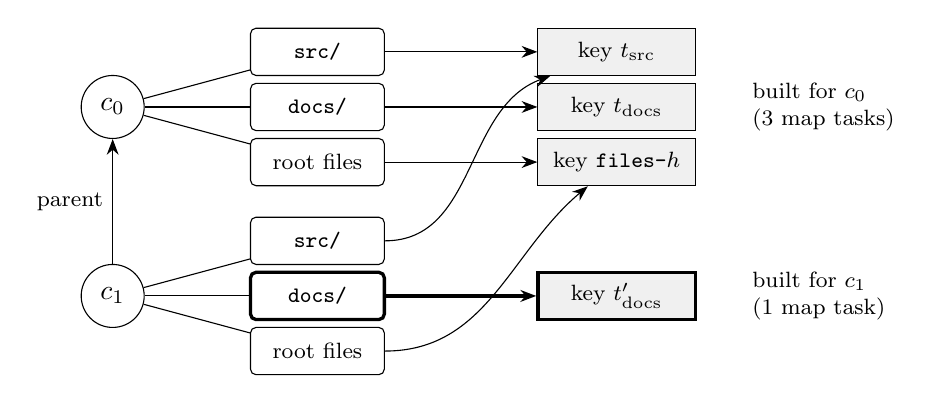
\begin{tikzpicture}[
  commit/.style={circle,draw,minimum size=8mm,inner sep=0pt},
  part/.style={rectangle,draw,rounded corners=2pt,minimum width=17mm,minimum height=6mm,font=\footnotesize},
  seg/.style={rectangle,draw,fill=black!6,minimum width=20mm,minimum height=6mm,font=\footnotesize},
  >={Stealth[length=2mm]}]
\node[commit] (c0) at (0,0) {$c_0$};
\node[commit] (c1) at (0,-2.4) {$c_1$};
\draw[->] (c1) -- node[left,font=\footnotesize]{parent} (c0);
\node[part] (s0) at (2.6,0.7) {\code{src/}};
\node[part] (d0) at (2.6,0) {\code{docs/}};
\node[part] (r0) at (2.6,-0.7) {root files};
\node[part] (s1) at (2.6,-1.7) {\code{src/}};
\node[part,very thick] (d1) at (2.6,-2.4) {\code{docs/}};
\node[part] (r1) at (2.6,-3.1) {root files};
\draw (c0) -- (s0); \draw (c0) -- (d0); \draw (c0) -- (r0);
\draw (c1) -- (s1); \draw (c1) -- (d1); \draw (c1) -- (r1);
\node[seg] (ks) at (6.4,0.7) {key $t_{\mathrm{src}}$};
\node[seg] (kd) at (6.4,0) {key $t_{\mathrm{docs}}$};
\node[seg] (kr) at (6.4,-0.7) {key \code{files-}$h$};
\node[seg,very thick] (kd2) at (6.4,-2.4) {key $t'_{\mathrm{docs}}$};
\draw[->] (s0) -- (ks); \draw[->] (d0) -- (kd); \draw[->] (r0) -- (kr);
\draw[->] (s1) to[out=0,in=200] (ks);
\draw[->] (r1) to[out=0,in=220] (kr);
\draw[->,very thick] (d1) -- (kd2);
\node[font=\footnotesize,align=left,anchor=west] at (8.0,0) {built for $c_0$\\(3 map tasks)};
\node[font=\footnotesize,align=left,anchor=west] at (8.0,-2.4) {built for $c_1$\\(1 map task)};
\end{tikzpicture}
\caption{Partition reuse for the test repository of Section~\ref{sec:pdd:evidence}. Commit $c_1$ changes only \code{docs/}, so two of its three partition keys already name stored segments and one map task runs. A query pinned at $c_0$ runs none.}
\label{fig:pdd:reuse}
\end{figure}

\begin{corollary}[Commit-keyed memoization]
\label{cor:pdd:commitkeyed}
Let a kind assign each pair $(c,p)$ of a commit and a path a value $g(c,p)$ that is a function of the ancestry of $c$ and the contents along it, and store $g(c,p)$ under the key $(\id(c),p)$ with a deterministic $g$ and the discipline of Assumption~\ref{as:pdd:store}. Then every value read from the store equals $g(c,p)$, for any interleaving of writers.
\end{corollary}

\begin{proof}
The proof of Theorem~\ref{thm:pdd:incremental} uses determinism, sufficiency and the store discipline, and never the form of a partition. Replace partitions by pairs $(c,p)$, $f_\delta$ by $g$ and $\kappa$ by $(c,p)\mapsto(\id(c),p)$ in the proof of Theorem~\ref{thm:pdd:incremental}. Sufficiency of this key is Lemma~\ref{lem:pdd:ancestry}: equal commit ids give equal ancestries and contents, hence equal values of $g$.
\end{proof}

\section{Search as a partitioned read job}
\label{sec:pdd:search}

Search is the derivation kind with the clearest Spark structure. The companion paper compares semantic indexing to Splunk's distributed search, in which a search head dispatches a query to search peers and assembles their results \cite{long2026inversion}. In YonedaRepo the head is the Worker invocation that handles the query and the peers are the stored segments; there is no separate peer process. The head plans the partitions of the commit's root tree, obtains each segment, asks the Rust \code{search\_segment} operation for candidates in each, filters candidates by the caller's grant before any candidate's content is read for matching, reads each remaining candidate blob and matches lines, and concatenates results in partition order up to a limit of 200, 50 by default. Building a segment reads every blob of its partition regardless of who asked; the grant governs what a query returns, not what the index contains.

The index follows Cox's design for regular-expression search with trigrams \cite{cox2012trigram}, restricted to literal queries. It is sound for indexed files.

\begin{proposition}[Candidate superset]
\label{prop:pdd:superset}
Let $q$ be a query that the adapter accepts (2 to 200 UTF-16 code units) and $F$ an indexed file of a segment. If the bytes of $F$ with ASCII letters folded to lower case contain the bytes of $q$ folded the same way, then $F$ is among the candidates the segment returns for $q$.
\end{proposition}

\begin{proof}
The code folds ASCII case byte by byte in both the content and the query and extracts the set of three-byte windows that contain no newline byte. If the folded query has no such window, which happens when no newline-free run of the query is three bytes long and in particular for any query of at most two bytes, the content filter is absent and every indexed file is a candidate. Otherwise every window of the folded query occurs inside the folded content of $F$, because a substring's windows are windows of the containing string and the newline filter treats both the same way. So $F$ appears in the posting list of every window of the query and in their intersection.
\end{proof}

Search is complete only for ASCII-folded matches in indexed files of indexed partitions. Both the trigram extractor and the line matcher fold case on ASCII bytes alone, so a query that differs from the content in the case of a non-ASCII letter does not match. Binary files and files over 1~MiB are never content candidates and match only by path. A partition with more than 20,000 files has no segment and is reported to the caller in \code{skipped\_partitions}.

Within those bounds the reduce returns exact matches, in partition order and in each segment's file order, up to the limit. Each candidate is narrowed by exact line matching on its verified blob. When matches exceed the limit, which of them are returned therefore depends on how the repository is partitioned.

\section{The prefix defect in the search key}
\label{sec:pdd:prefix}

The search view in the reference implementation is not consistent at every snapshot. The search map function records each file's full path, including the partition prefix. The key of a directory partition is the bare subtree id. Listing~\ref{lst:pdd:key} shows the two lines that fix the key, from \code{plan} in \path{platform_derived.rs} and \path{repo-derived.ts}.

\begin{lstlisting}[caption={The partition key in the plan (Rust) and the storage key (TypeScript) at commit \code{cfa4845}.},label={lst:pdd:key}]
// backend/crates/yoneda-platform/src/platform_derived.rs, fn plan
.map(|e| json!({ "prefix": e.name, "tree": e.id, "key": e.id, "shallow": false }))

// cloudflare/worker/repo-derived.ts
const segmentKey = (repo: string, key: string) => `derived/v1/${repo}/search/${key}`;
\end{lstlisting}

\begin{proposition}[Prefix-free keys are insufficient for search]
\label{prop:pdd:prefix}
Let $f_{\mathrm{s}}$ be the implemented search map function and $\kappa(d,x)=\id(x)$ the implemented key for directory partitions. If two directory partitions $(d,x)$ and $(d',x)$ with $d\ne d'$ cover the same nonempty subtree $x$, in one commit or in two, then $\kappa(d,x)=\kappa(d',x)$ and $f_{\mathrm{s}}(d,x)\ne f_{\mathrm{s}}(d',x)$. So $\kappa$ is not sufficient for $f_{\mathrm{s}}$.
\end{proposition}

\begin{proof}
The keys are equal by definition. The segment $f_{\mathrm{s}}(d,x)$ lists every file of $x$ under a path beginning with $d/$, while $f_{\mathrm{s}}(d',x)$ lists the same files under paths beginning with $d'/$. Since $x$ contains at least one file, the two path lists differ.
\end{proof}

The hypothesis is met in ordinary repositories. Two top-level directories that each hold only an empty placeholder file have the same tree id by Lemma~\ref{lem:pdd:merkle}. So do two vendored copies of one library, and so does a single directory before and after a rename that leaves its content alone. Proposition~\ref{prop:pdd:necessity} then applies, and the consequences follow from the code.

Prefix-free keys misattribute paths after a directory rename, and the misattribution defeats Part~I's grant invariant~I14 at the queried commit (Part~I, Table~3). When \code{src/} is renamed to \code{lib/} without content changes, queries at the new commit reuse the segment built for \code{src/} and report hits under \code{src/\ldots} paths that do not exist in that commit. The matched lines are still correct, because \code{grep} reads each candidate by blob id. Grant filtering in \code{keepAllowed} uses the stored paths, not the paths at the queried commit. A caller whose grant covers \code{src/} but not \code{lib/} therefore receives matches from files that exist only under \code{lib/}, and a caller whose grant covers only \code{lib/} receives none.

How far the harm extends depends on where the stored segment came from. Segment keys are scoped to one repository, and directory grants restrict paths at every commit (Part~I, invariant~I14), so the leaked bytes always existed under the reported path in some commit of the same repository. When that commit is an earlier commit on a branch the caller can read, only the attribution is wrong. When it is a commit the caller cannot discover, such as unlanded work of another writer, the caller receives content it had no practical way to reach.

Prefix-free keys also corrupt results within one commit whenever two top-level directories \code{a/} and \code{b/} have identical content. On a cold store, the first query builds a segment for each directory with its own prefix and returns correct paths, but both writes target one R2 key. Every later query reads the one stored segment for both partitions and reports each match twice under one prefix and never under the other. Two writes to one key within a second can also exceed R2's per-key write limit \cite{cfr2limits}; we have not observed this.

Prefix-free keys make a codemod either fail permanently or leave a directory unedited. After the rename of \code{src/} to \code{lib/}, the codemod reads the stale segment and emits changes for \code{src/\ldots} paths, each with an expected old blob. The parent tree has no such paths, so commit preparation rejects the commit with \code{CONFLICT} (\path{prepare.rs}), and it does so on every retry because the stored segment never changes. With duplicated directories, the reduce receives two identical changes for each matching path under one prefix and none under the other, so either the commit is refused or one directory is left unmodified.

A test confirms the key collision; no test in the repository covers it. We wrote the test against the Rust crates at commit \code{cfa4845} and ran it outside the repository (Appendix~\ref{app:pdd:prefixtest}). For a commit with identical top-level directories \code{a/} and \code{b/}, and for a rename of \code{src/} to \code{lib/}, it asserts that \code{search\_plan} gives both partitions the same key and that \code{index\_partition} builds segments listing different paths. It also asserts that stripping each segment's prefix makes the segments equal. The effects on search responses and codemods follow from the TypeScript adapter, which passes the plan's key unchanged to R2 (Listing~\ref{lst:pdd:key}); we traced them by reading that code and did not run the adapter.

\begin{proposition}[Two repairs]
\label{prop:pdd:repairs}
Each of the following restores sufficiency for directory partitions. (a) Keep $f_{\mathrm{s}}$ and use the key $\kappa_a(d,x)=H(d\,\|\,\id(x))$. (b) Use a map function $f_{\mathrm{r}}(x)$ that records paths relative to the partition root, keep $\kappa(d,x)=\id(x)$, and let the reduce prepend $d/$ to every path of the segment for partition $(d,x)$.
\end{proposition}

\begin{proof}
For (a), $\kappa_a(d,x)=\kappa_a(d',x')$ implies $d=d'$ and $\id(x)=\id(x')$ by collision resistance of $H$ and the fixed-width encoding of ids, hence $x=x'$ by Lemma~\ref{lem:pdd:merkle}, so $f_{\mathrm{s}}(d,x)=f_{\mathrm{s}}(d',x')$. For (b), $f_{\mathrm{r}}$ depends only on $x$, and $\id(x)=\id(x')$ implies $x=x'$. The reduce sees each segment together with the prefix of its partition, as in Definition~\ref{def:pdd:kind}, so the prefixed result equals $f_{\mathrm{s}}(d,x)$.
\end{proof}

Repair (b) is the better one. It keeps the reuse across renames, vendored copies and forks that Proposition~\ref{prop:pdd:fixpoint}(c) describes, and its cost is one string concatenation per reported path. Repair (a) is a one-line change but gives up that reuse. Either repair needs a new key namespace, because existing segments were built under the old function (Remark~\ref{rem:pdd:versions}).

\begin{remark}[Versioned keys]
\label{rem:pdd:versions}
A store that outlives a change of map function from $f$ to $f'$ satisfies Assumption~\ref{as:pdd:store}(ii) for $f'$ only if keys written under $f$ are unreachable from $f'$. Mononoke encodes this in its key names, for example \code{derived\_root\_blame\_v2} \cite{mononokederived}. YonedaRepo encodes it as a literal path component: \path{derived/v1/} for search and \path{symbols/v1/} for symbol tables. The symbol extractor also carries a constant \code{EXTRACTOR\_VERSION} whose comment asks for it to be bumped when output changes. The constant is stored inside each table, but the key does not contain it, and the reader does not compare it. A bump of the constant without a change of the literal would serve stale tables.
\end{remark}

Symbol tables illustrate a weaker form of sufficiency that the theorem also covers. A table is keyed by file extension and blob id, and it contains the path of the file it was first built for. Two files with equal content and extension share a table that names only one of them. The readers in \path{repo-code.ts} never use the stored path; they take the path from the request. If $\pi$ is the projection that discards the stored path, the key is sufficient for $\pi\circ f$, and Theorem~\ref{thm:pdd:incremental} holds for every answer computed through $\pi$. The search reduce, by contrast, does use the stored paths, which is why the prefix defect is visible.

\section{History, checks and seeds}
\label{sec:pdd:history}

Blame and path history are not functions of the tree. Two commits with the same tree can have different histories, so no tree id is a sufficient key for them. The commit id is, by Lemma~\ref{lem:pdd:ancestry}.

Any kind whose value at $c$ is a function of the ancestry of $c$ and the contents along it therefore has the commit id as a sufficient key, and Corollary~\ref{cor:pdd:commitkeyed} gives correct memoization under that key. Mononoke keys its derived roots by changeset id \cite{mononokederived}, which is the same choice.

Path history is computed by \code{path\_history} in \path{history.rs}. It walks the first-parent chain from the head of a ref, at most 5,000 commits, and returns each commit whose recorded touches overlap the requested path or prefix, newest first. It reads the changed-path rows written with each commit and no trees. Its value at $(c,p)$ is a function of the first-parent chain of $c$, so $(\id(c),p)$ is a sufficient key. Nothing is stored, so each query pays for the walk.

Blame is computed by \code{blame} in \path{blame.rs} from the versions of a file along that chain, oldest first. Let $v_0,\ldots,v_m$ be the file's contents at the commits $c_0,\ldots,c_m$ that changed it, and let $\mathrm{own}_i$ be the vector that assigns each line of $v_i$ the commit that last changed it.

\begin{proposition}[Blame is a fold]
\label{prop:pdd:blame}
Let $v_0,\ldots,v_m$ be the complete sequence of versions of the file along the first-parent chain, without the implementation's window. Define $\mathrm{own}_0=(c_0,\ldots,c_0)$ with one entry per line of $v_0$, and obtain $\mathrm{own}_{i+1}$ from $\mathrm{own}_i$ by copying the owners of lines outside the hunks of the line diff from $v_i$ to $v_{i+1}$ and assigning $c_{i+1}$ to every line inside a hunk. Then $|\mathrm{own}_i|$ equals the number of lines of $v_i$ for every $i$, and \code{blame} returns $\mathrm{own}_m$ paired with the lines of $v_m$. Consequently blame satisfies the parent-recursive form of Definition~\ref{def:pdd:fold}: if $c$ changes the file relative to its first parent $c'$, then $\mathrm{Blame}(c)=\mathrm{update}(\mathrm{Blame}(c'),\mathrm{diff}(v(c'),v(c)),c)$, and otherwise $\mathrm{Blame}(c)=\mathrm{Blame}(c')$.
\end{proposition}

\begin{proof}
The hunks of a line diff are disjoint, ordered by position, and together with the unchanged runs they partition the old lines and the new lines. For each hunk, the code copies the owners of the unchanged old lines before it, then appends one owner per new line of the hunk, and after the last hunk copies the remaining owners. The number of entries appended equals the number of new lines, which proves the length claim by induction. The recursive form restates one step of the induction; since $\mathrm{Blame}(c')$ pairs $\mathrm{own}_{m-1}$ with the lines of $v(c')$, the update is a function of $c$ and $\mathrm{Blame}(c')$ alone, as Definition~\ref{def:pdd:fold} requires.
\end{proof}

The implementation evaluates the fold from scratch at every query, so a blame costs one diff per version of the file, over the newest versions that the request reads from path history: 200 by default, and at most 1,000 because path history caps its limit. Versions older than that window are attributed to the oldest version kept, which acts as a history boundary in the manner of \code{git blame}'s caret.

The proposition describes the untruncated fold. With the window, the oldest kept version moves as new versions arrive, so the windowed blame of $c$ is not an update of the windowed blame of $c'$. Memoizing the untruncated fold under the key $(\id(c),p)$ would remove the window and reduce the cost to one diff per landed change to the file, and Corollary~\ref{cor:pdd:commitkeyed} makes that memoization correct. This is the recursive blame the Scion post describes \cite{anthropic2026scion}, and YonedaRepo does not yet have it.

Blame and path history also follow only the first parent. Changes reached only through a merge's other parents are attributed to the merge, and neither computation follows renames.

Rename detection is change-local and exact. The tree diff pairs a deleted file and an added file with the same blob and mode into one rename, which matches \code{git diff -M100\%} (\code{with\_renames} in \path{platform_compute.rs}). A rename with any edit is reported as a deletion and an addition. Copy detection is not implemented.

Check results are derived data with a policy in the key. A run is bound to the exact commit, the check name and the digest of the landing policy, and only completions from the run's current epoch count (\path{checks.rs}). Changing the policy changes the digest, so results recorded under the old policy stop counting for gates. The key $(\id(c),\text{check},\text{digest})$ is sufficient only for a deterministic runner. A flaky test makes the result an observation rather than a function, and reusing it is a policy choice that the theorem does not justify.

Bisect uses check results as its oracle. Given a good commit $g$ and a bad commit $b$ on one branch, its candidates are the first-parent commits after $g$ up to $b$, at most 10,000 (\path{bisect.rs}). Each step reads the check result at the midpoint, requesting a run if none exists under the current policy, and halves the range.

\begin{proposition}[Bisect]
\label{prop:pdd:bisect}
Let $x_1,\ldots,x_n$ be the candidates, with $x_n=b$ taken as failing without a run, and suppose the check is deterministic and monotone along the chain: once it fails at some $x_i$, it fails at every $x_j$ with $j\ge i$, and it passes at $g$. Then bisect returns the first failing candidate after at most $\lceil\log_2 n\rceil$ check executions on candidates.
\end{proposition}

\begin{proof}
The invariant is that the first failing candidate lies in the current range $(\ell,u]$, where the check passes at $\ell$ (initially $g$) and fails at $u$ (initially $x_n$). Testing the midpoint and replacing $\ell$ or $u$ by it preserves the invariant by monotonicity and halves the number of candidates in the range, rounding up. After $\lceil\log_2 n\rceil$ steps the range contains one candidate, which is the first failure. Results that already exist under the policy digest are reused and cost no execution, so the bound counts at most one execution per step.
\end{proof}

The repository's test bisects seven candidates with an injected regression at the fourth and asserts at most three executions on candidate commits and the correct answer (Section~\ref{sec:pdd:evidence}). Without monotonicity the procedure still terminates at a boundary where a passing candidate precedes a failing one, but that boundary need not be the first regression.

Warm-start seeds are a content-local kind computed eagerly. After a landing, the derivation job writes to R2 one object containing every file at the branch head, and a check run on a nearby commit starts from the seed and fetches only the blobs that differ (\path{repo-seed.ts}). A seed write that fails costs only speed.

Seeds are the one derived kind with a measured benefit, and the measurement is thin. The commit that introduced seeds reports that a seeded hosted check run on a nearby commit of a 301-file repository fetched 1 of 301 blobs % M37
and took 8.1~s against 109~s for the first cold run, most of which was Container start. % M35
The same commit reports 1 against 201 blob fetches in the local test. % M66
These three figures come from a commit message and have no raw output on disk.

\section{Write jobs}
\label{sec:pdd:write}

\begin{definition}[Write job]
\label{def:pdd:writejob}
A write job over commit $c$ at log version $v$ is a job whose map function sends each partition $(p,x)$ to a set $C_p$ of file changes below $p$ and whose reduce forms the single commit with parent $c$, base version $v$ and change set $C=\bigcup_p C_p$. The commit then lands through Part~I's validation (Part~I, Definition~4.15).
\end{definition}

The implemented write job is the literal codemod in \code{codemod} in \path{repo-code.ts}. It obtains the search segments of the head, takes in each partition the candidate files for the find string that the caller's grant allows and that lie under an optional path prefix, and asks the Rust \code{replace\_literal} operation to replace every non-overlapping occurrence in each candidate. A changed file becomes a change carrying the new content and the old blob id as its expected value. The reduce concatenates the changes and creates one commit on the head, with the head's version as base. It does not land the commit.

\begin{proposition}[Codemod reduce]
\label{prop:pdd:codemod}
Assume the search key is sufficient (Section~\ref{sec:pdd:prefix}). Then: (a) the sets $C_p$ are pairwise disjoint in paths, so $C$ contains at most one change per path; (b) every expected blob id in $C$ matches the parent tree, so commit preparation accepts $C$; (c) the job creates either one commit containing all of $C$ or no commit; and (d) two runs with the same head, find string, replacement, prefix and grant produce the same tree, although their commit ids may differ.
\end{proposition}

\begin{proof}
(a) Each $C_p$ contains only paths below $p$, and partitions of one commit are disjoint in paths. (b) By Theorem~\ref{thm:pdd:incremental} the segments are those of the head, so each candidate's blob id is the head's blob at that path, and \code{replace\_literal} returns that id as the expected value. (c) All partitions run under one \code{Promise.all}; any failure rejects the request before the single call that creates the commit. Commit preparation is itself all or nothing, and the commit enters the log as one entry, as a Delta transaction commits as one log record \cite{armbrust2020delta}. (d) The replacement is a deterministic function of the blob and the arguments, the candidate set is a deterministic function of the segments and the grant, and the tree of a commit is determined by its parent's tree and its changes. The commit object also carries the request time in seconds, so its id need not repeat.
\end{proof}

The codemod's result is complete only for indexed files. A file over 1~MiB is never a candidate and is never rewritten, and a partition over 20,000 files is skipped. The codemod's response reports the number of partitions but not which were skipped, so a caller cannot tell that the replacement was partial.

Rerunning a codemod on its own output changes nothing exactly when the output contains no occurrence of the find string. The repository's test checks the empty case: a codemod for a string that occurs nowhere returns \code{changed: false}.

A codemod that declares no read set admits write skew under backward validation. A codemod reads every candidate in every scanned partition, and its result depends on the absence of the find string elsewhere. The commit it creates declares no read set. Under Part~I's backward validation, an entry that landed after version $v$ and touched one of the codemod's files is a write-write overlap, which leads to a content merge rather than a conflict, and an entry that touched only other files leads to a rebase (Part~I, Definition~4.15). In both cases the codemod lands. A file that gained an occurrence of the find string after version $v$ is not rewritten, and the landed tree contains the old string. This is write skew in the sense of Berenson et al.: each transaction is valid against a snapshot, and their combination is not equivalent to any serial order \cite{berenson1995critique}.

The codemod at commit \code{cfa4845} neither accepts nor declares a read set, so Proposition~\ref{prop:pdd:serializable} below characterizes a proposed extension of its commit request. Declaring a directory as a read is a predicate read in the sense of Fekete et al.\ and Adya: a read of every item that satisfies a predicate, here every path below the directory, including paths added later \cite[Definition~2.1]{fekete2005serializable} \cite{adya1999thesis}. Delta Lake's conflict checker performs the corresponding test, failing a transaction when a concurrent commit added files that match its partition read predicates \cite{deltaconflictsrc}; the difference is that Delta derives the predicate from the query, while here the writer declares it.

\begin{proposition}[Serializable codemods]
\label{prop:pdd:serializable}
Assume the search key is sufficient. Let a codemod over version $v$ be restricted to a directory prefix $q/$, so that it reads and writes only paths below $q/$, and let it declare the read set $\R=\{q/\}$. Suppose that the top-level partition containing $q/$ is within the indexing cap of 20,000 files at $v$ and also immediately before the landing; the second condition follows from the first when $q/$ is itself a top-level directory. If its commit lands by itself, or in a combiner batch that satisfies the acceptance rule of Part~I, Proposition~7.4, the landed tree below $q/$ equals the codemod applied to the snapshot immediately before its landing.
\end{proposition}

\begin{proof}
By (P1), validation returns a conflict, and the landing is refused, whenever an entry after $v$ on the same ref has a refined write that overlaps $\R$. Every path below $q/$, including a path added after $v$, and every symbol of a file below $q/$ overlaps $q/$. So a landing succeeds only if no entry after $v$ touched a path below $q/$, and then the subtree at $q/$ is the same immediately before the landing as at $v$. Because the enclosing partition is indexed at both versions and the key is sufficient, the codemod applied to that snapshot computes the same candidates below $q/$ and the same changes. When $q/$ is top level, its partition's size changes only through writes below $q/$, which validation refuses, so a partition within the cap at $v$ is still within it. By (P2), the landed tree equals the pre-landing tree with the codemod's changes applied on its write set, which is the claim. Inside a batch, the acceptance rule in (P3) makes the batch equivalent to landing its members one at a time in ticket order, and the same argument applies to each.
\end{proof}

Without the batch condition a declared read does not protect a codemod. By (P3), the combiner at commit \code{cfa4845} validates batch members against the log but not against each other. A codemod that shares a batch with a commit adding an occurrence of the find string in its scope would land, and the new occurrence would survive.

A repository-wide codemod cannot be made serializable by declaring reads. Such a codemod scans every top-level directory and the root files, and a declared set of those directory prefixes and file paths does not cover a top-level directory or root file added after $v$. A concurrent commit that adds such a file containing the find string writes nothing the codemod declared, validation returns a rebase, and the new occurrence survives. Part~I's access entries have no form that covers the whole repository, so the only condition that makes a repository-wide codemod serializable is that its landing be a fast-forward, with no entry on the ref after $v$. Declared reads also cost refusals. Any concurrent landing in scope forces the codemod to rerun, and the rerun is the only way to rewrite a new occurrence.

Retrying only a failed partition requires memoizing the codemod's map outputs. The design notes promise that a failed partition is retried alone. The code reruns the whole job, which re-reads segments from the store but repeats every replacement. Memoizing the map outputs gives partition-level retry with the same correctness argument.

\begin{proposition}[Partition-level retry]
\label{prop:pdd:retry}
Store each $C_p$ under the key
\[
\bigl(\textsf{codemod},\;H(\langle\text{find},\text{replace},\text{prefix},\text{grant},p\rangle),\;\kappa(p,x)\bigr),
\]
where $\langle\cdot\rangle$ encodes the tuple with a length prefix on each component, and with $\kappa$ sufficient for search. Then a retry that reuses stored $C_p$ and recomputes only missing ones produces the same $C$ as a fresh run on the same head.
\end{proposition}

\begin{proof}
$C_p$ is a deterministic function of the partition content, the arguments and the grant. The length-prefixed encoding is injective, so by Assumption~\ref{as:pdd:collision} the digest determines the four arguments and the partition prefix $p$, and $\kappa$ determines the subtree. The prefix is needed: $C_p$ lists full paths and is filtered by the job's prefix and grant, so two partitions with the same subtree under different prefixes have different outputs, which is the defect of Section~\ref{sec:pdd:prefix} in another form. This is idempotent re-execution of a deterministic task \cite[Section~3.3]{dean2004mapreduce}, the purpose that Delta's transaction identifiers serve for writes \cite{deltaprotocol}. Theorem~\ref{thm:pdd:incremental} applies with this key and map function.
\end{proof}

The grant must be part of the key because candidate filtering depends on it. Omitting it would let one caller's stored changes be reused for a caller with a narrower grant, which is the same defect as in Section~\ref{sec:pdd:prefix} with an access-control consequence. Partition-level retry is not implemented.

\section{Semantic partitioning and the plan DAG}
\label{sec:pdd:plan}

Directory partitions organize derived data. Agent work needs a finer partition. The companion paper separates the maintenance plan, a DAG over work items, from the program's dependency graph, which may have cycles, and requires cyclically dependent changes to be grouped into a joint stage \cite{long2026inversion}. YonedaRepo implements this as a planning operation over symbol-level read and write sets (\path{txlog/plan.rs}, exposed as \code{POST /plans}). The platform plans; it does not run the work.

\begin{definition}[Plan inputs]
\label{def:pdd:plan}
A work item is a tuple $(i,b_i,\R_i,\W_i)$ of an id, an optional base version and declared read and write sets of path, prefix and symbol entries (Part~I, Definition~4.4). The symbol graph at the plan revision is a directed graph $G_s=(N,E)$ whose nodes are symbols $(\text{path},\text{symbol path})$ and whose edges point from a symbol to the symbols it references, together with a set $\mathcal{C}$ of coarse files whose symbols are unknown; no node of $N$ lies in a file of $\mathcal{C}$. For an access set $A$, $\mathrm{cov}(A)\subseteq N$ is the set of nodes it covers: every symbol of every file that a path or prefix entry of $A$ overlaps, and every symbol named by a symbol entry together with its nested members. An item \emph{writes} the nodes in $\mathrm{cov}(\W_i)$ and \emph{touches} the nodes in $\mathrm{cov}(\R_i\cup\W_i)$.
\end{definition}

Before planning, the method \code{AccessSet::coarsen} replaces every symbol entry on a coarse file by the whole path. This is Part~I's coarsening rule (Part~I, Proposition~6.10). The planner then runs four steps.
\begin{enumerate}
\item \emph{Join.} Compute the strongly connected components of $G_s$ with an iterative form of Tarjan's algorithm \cite{tarjan1972}. For each component with more than one node, if some item writes a node of it and at least two items touch it, merge all items that touch it into one joint item, using union-find. A joint item's read and write sets are the unions of its members' coarsened sets.
\item \emph{Closure.} Add to each joint item's reads the symbols reachable from the nodes it touches by following at most $d$ reference edges forward, where $d$ is the requested closure depth. Call the result its effective reads $\hat{\R}$.
\item \emph{Order.} Let item $k$ feed item $l$ when $\W_k\bowtie\hat{\R}_l$. Compute the components of the feed relation with Tarjan's algorithm and order the items topologically over their condensation, breaking ties between components by the smallest input position of their members and ordering the members of one component by input position. Every choice depends only on input positions.
\item \emph{Stage.} Process items in that order. For each item $l$, set its stage to one more than the largest stage of any earlier item $k$ that is not independent of $l$ under the effective sets, and record $k$ in the list of items $l$ must follow; items with no such predecessor get stage 0.
\end{enumerate}

\begin{theorem}[Plan properties]
\label{thm:pdd:plan}
For any inputs, the plan returned by \code{plan} satisfies the following.
\begin{enumerate}
\item[(a)] Every input item belongs to exactly one joint item.
\item[(b)] Two distinct joint items in the same stage are independent under their effective read sets and write sets.
\item[(c)] For every pair of distinct joint items that are not independent, one is in the other's list of predecessors and has a smaller stage.
\item[(d)] If joint item $k$ feeds joint item $l$ and they lie in different components of the feed relation, then $\mathrm{stage}(k)<\mathrm{stage}(l)$.
\item[(e)] The stage of an item is the number of items on the longest chain of predecessors ending at it, minus one. With unit durations and at least as many workers as the largest stage size, executing the stages in order finishes in exactly as many time units as there are stages, which equals the critical-path term of the companion paper's \cite[Eq.~2]{long2026inversion} bound for the DAG of recorded predecessor edges.
\end{enumerate}
\end{theorem}

\begin{proof}
(a) Union-find starts with one class per input item and only merges classes, and the joint items are its final classes.
(b) and (c). Let $k$ precede $l$ in the processing order. If they are not independent, the stage step records $k$ as a predecessor of $l$ and sets $\mathrm{stage}(l)\ge\mathrm{stage}(k)+1$. Independence is symmetric, as the property test \code{eq1\_is\_symmetric} checks and as the definition makes evident. So every non-independent pair is ordered, with strictly increasing stage, and no two such items share a stage.
(d) The order step places every component of the feed relation before the components it feeds. So $k$ precedes $l$. Feeding means $\W_k$ overlaps $\hat{\R}_l$, so the pair is not independent, and (c) gives the inequality.
(e) The stage step computes $\mathrm{stage}(l)=\max\{\mathrm{stage}(k)+1\}$ over predecessors, with 0 for none, and it processes predecessors before successors. This is the longest-path layering of the predecessor DAG, so $\mathrm{stage}(l)+1$ is the length in items of the longest chain ending at $l$. Items in one stage are independent by (b) and all their predecessors lie in earlier stages, so with enough workers each stage takes one time unit. The longest chain has as many items as there are stages, so the critical-path term of the bound equals the number of stages, and the schedule meets the bound.
\end{proof}

The planner groups cycles more narrowly than the companion paper's instruction to group cyclic dependencies might suggest. It joins items only on a component that some item writes and that at least two items touch. Items that only read a cycle are not joined, which the test \code{readers\_alone\_do\_not\_join\_a\_cycle} checks. The plan therefore has one work item per written cycle of two or more symbols shared by several items, not one per strongly connected component of the program. Items that feed each other through their declared sets, without sharing a written symbol cycle, are not joined either. Step 3 places them in input order and step 4 gives them different stages, so the later one is planned to read the earlier one's writes. Joining is reserved for reference cycles in the program, which no order of edits can break, while a feed cycle between declared sets is broken by choosing an order. A symbol that references itself forms no such component; two items that touch it, one of them writing it, overlap directly and are ordered into different stages by step 4.

\begin{proposition}[Fewest stages is graph coloring]
\label{prop:pdd:coloring}
Let $H$ be the undirected conflict graph whose vertices are joint items and whose edges join pairs of distinct items that are not independent. Apply the staging rule of step 4 to an arbitrary processing order of the vertices. The resulting stages form a proper coloring of $H$, and for every proper coloring of $H$ with $\chi$ colors there is a processing order under which the rule produces at most $\chi$ stages. The fewest stages over all processing orders therefore equals the chromatic number of $H$.
\end{proposition}

\begin{proof}
For any processing order, two adjacent vertices are not independent, so the later one receives a stage larger than the earlier one's, by the argument for Theorem~\ref{thm:pdd:plan}(b); stages therefore color $H$ properly. Given a proper coloring with colors $0,\ldots,\chi-1$, process vertices in increasing color. A predecessor of $l$ is an adjacent vertex processed earlier, which has a strictly smaller color. By induction on color, a vertex of color $j$ receives a stage at most $j$, so the plan has at most $\chi$ stages.
\end{proof}

The proposition is the Gallai-Hasse-Roy-Vitaver theorem applied to the staging rule: the layers of the longest-path layering of an acyclic orientation color the graph properly, and some acyclic orientation has exactly $\chi(H)$ layers \cite[Th\'eor\`emes~1 and~2]{roy1967}. Each processing order induces an acyclic orientation of $H$, and every acyclic orientation arises from a topological order, so the proof above is the reduction. Minimizing the number of stages over all orders is as hard as graph coloring, which is NP-complete in its decision form (see \cite{karp1972}). The planner's fixed order is a greedy coloring. The choice is defensible for a scheduler that must be deterministic and fast, but the stage count it reports is an upper bound on the parallel depth, not the minimum.

The planner does not range over all orders. Step 3 places a writer before every item it feeds whenever the two lie in different components of the feed relation, so the planner's minimum is at least the chromatic number and can exceed it. Statement (e) of Theorem~\ref{thm:pdd:plan} is therefore optimal only for the predecessor DAG that the planner chose, and a different orientation of the conflicts could give fewer stages.

The cost of planning is dominated by the stage step. With $m$ joint items it tests independence for $m(m-1)/2$ ordered pairs, and each test compares entries pairwise, so the step is quadratic in the number of items and quadratic in the size of their sets. Tarjan's algorithm is linear in $|N|+|E|$ \cite{tarjan1972}. The planning request also diffs the plan revision's whole tree against the empty tree to list the files from which the symbol graph is built (\path{repo-plan.ts}), so its object reads grow with the repository, not with the plan.

The companion paper proves that a pure physical repartition, which moves semantic units between files without changing the semantic graph or the edit core, leaves the semantic closure unchanged \cite{long2026inversion}. The planner inherits this property only under a condition on how items are declared.

\begin{proposition}[Representation invariance of plans]
\label{prop:pdd:invariance}
Write $u\sqsubseteq w$ for symbols $u,w$ when they lie in the same file and the symbol path of $u$ equals or is nested in that of $w$. Let $\varphi$ be a bijection between the symbols of two repository layouts such that $(u,w)\in E$ if and only if $(\varphi(u),\varphi(w))\in E$, and $u\sqsubseteq w$ if and only if $\varphi(u)\sqsubseteq\varphi(w)$. Extend $\varphi$ to symbol access entries that name nodes of $N$. If every entry of every work item is a symbol entry naming a node of $N$ and no file containing a covered symbol is coarse in either layout, then the plan for the relabeled items over the relabeled graph is the relabeling of the original plan: the same joins, closures, order and stages.
\end{proposition}

\begin{proof}
Each planning step reads the inputs only through covered node sets, reference edges, component membership and the overlap of symbol entries. For symbol entries, overlap holds exactly when $u\sqsubseteq w$ or $w\sqsubseteq u$. A bijection that preserves and reflects edges and $\sqsubseteq$ therefore preserves and reflects overlap, covered sets and components, and coarsening does not occur by hypothesis. The reflection matters: a layout that merges two files can create an overlap that did not exist before, and a map that only preserved $\sqsubseteq$ would miss it. Each step is therefore equivariant under $\varphi$, and so is their composition.
\end{proof}

The hypotheses are not decorative. A path entry covers every symbol of a file, so moving a symbol into or out of the file changes what the entry covers and can change the plan. A coarse file turns symbol entries into path entries, with the same effect. The relation $\sqsubseteq$ is preserved and reflected when whole top-level items move between files. It is not when a layout spreads one type's members over several files, which Rust's multiple \code{impl} blocks permit, or merges files whose symbol paths are prefixes of one another, because symbol overlap requires the same file. A repository that wants plans independent of layout should therefore declare work at symbol granularity and keep its sources parseable.

\begin{definition}[Symbol handle]
\label{def:pdd:handle}
A handle is a tuple $h=(c,\text{path},\text{symbol path},\text{range},\text{digest})$ issued by a symbol read at commit $c$, where the digest is the platform digest of the symbol's bytes in that commit.
\end{definition}

\begin{proposition}[Stale handles are rejected]
\label{prop:pdd:stale}
A symbol edit with handle $h$ on the head of a ref is accepted only if the symbol named by the handle exists in the head's version of the file and the digest of its current bytes equals the handle's digest, and only if the edited file still parses. Under collision resistance of the digest, an accepted edit never overwrites a change to that symbol's text made after the handle was issued, except a change that restored identical bytes.
\end{proposition}

\begin{proof}
\code{symbol\_edit} in \path{platform_code.rs} looks up the symbol by its qualified path in the current file and returns \code{STALE\_HANDLE} if it is missing or if its digest differs, and it returns \code{INVALID\_EDIT} if the edited file does not parse. Equal digests imply equal bytes under collision resistance.
\end{proof}

The test for this property edits two symbols of one file. After another commit changes the first symbol and lands, an edit through the first symbol's old handle is refused with \code{STALE\_HANDLE}, and an edit through the second symbol's handle succeeds (Section~\ref{sec:pdd:evidence}).

The handle check protects an edit only until its commit is created. Between creation and landing, protection comes from Part~I's validation. The edit commit declares the whole file as its read set, so any later landing that touched the file, including a change to a different symbol, makes the edit's landing a stale read. Declaring \code{path\#symbol} instead would admit concurrent edits to different symbols of one file, at the price of trusting the symbol derivation of the other commit; Part~I's validation narrows a later entry's writes to symbols only when the platform derived them.

The symbol tables behind handles and plans are built by pure-Rust parsers, syn for Rust and oxc for TypeScript and JavaScript, running inside the Worker. The design notes had planned tree-sitter in Containers. The deviation buys determinism, local testing and the absence of a Container round trip, and it costs language coverage: only Rust, TypeScript and JavaScript files have symbols, and every other file is coarse. The platform's WebAssembly build, which includes these parsers, is 5.0~MB. % M68

\section{Partition granularity}
\label{sec:pdd:granularity}

Proposition~\ref{prop:pdd:cost} charges each evaluation one lookup per partition and each changed partition its full size. Coarse partitions make the second term large and fine partitions make the first term large. The companion paper's scalar granularity model has exactly this form \cite{long2026inversion}, and its finite-optimum proposition applies once the coefficients are identified.

\begin{proposition}[Optimal partition size]
\label{prop:pdd:granularity}
Consider a repository of $N$ files split into partitions of $g$ files each. Let derivation jobs run at rate $\tilde\lambda_c$, which is at most the landing rate because landings are coalesced, and let $u$ be the mean number of partitions a job rebuilds, independent of $g$. Let queries arrive at rate $\lambda_q$; let indexing cost $c_i$ per file and a lookup cost $c_\ell$ per partition. Suppose every derivation job and every query looks up all partitions, as the implemented evaluator does, and that queries find every segment already built by a job, so that only jobs rebuild. Then the expected derivation cost per unit time is
\[
C(g)=k+a\,g+\frac{b}{g},\qquad a=\tilde\lambda_c\,u\,c_i,\qquad b=(\tilde\lambda_c+\lambda_q)\,N\,c_\ell,
\]
and when $N$, $\tilde\lambda_c$, $u$, $c_i$ and $c_\ell$ are positive it has on $(0,\infty)$ the unique minimizer $g^*=\sqrt{b/a}$ with $C(g^*)=k+2\sqrt{ab}$. On a feasible interval the minimizer is the projection of $g^*$ onto it.
\end{proposition}

\begin{proof}
Jobs rebuild partitions of $g$ files at rate $\tilde\lambda_c u$, costing $\tilde\lambda_c\,u\,g\,c_i$ per unit time. By hypothesis, queries rebuild nothing. Each derivation job and each query performs $N/g$ lookups, costing $(N/g)\,c_\ell$. Multiplying the lookup cost by the job and query rates and collecting terms gives $C(g)$, where $k\ge 0$ collects the derivation costs that do not depend on $g$, such as reduces and line matching. The minimizer is the companion paper's finite-optimum result \cite[Eq.~19]{long2026inversion}, whose proof is the first-order condition $a-b/g^2=0$ and strict convexity.
\end{proof}

An evaluator that prunes derivation jobs by touched paths (Proposition~\ref{prop:pdd:pruning}) looks up only the $u$ changed partitions per job. Its lookup cost $\tilde\lambda_c\,u\,c_\ell$ does not depend on $g$ and moves into $k$. That leaves $b=\lambda_q N c_\ell$, which is smaller, so the optimum $g^*$ is smaller: when jobs stop paying a lookup per partition, finer partitions become cheaper.

The model is a structural hypothesis, as the companion paper says of its own scalar model. Its assumption that $u$ does not depend on $g$ fails for very small partitions, where a commit that touches several nearby files spans several partitions. Its value here is diagnostic. It says that the implemented rule, one partition per top-level directory, fixes $g$ by the repository's layout rather than by the rates and costs that determine $g^*$. A repository whose code sits under one top-level directory has a single partition, and every commit re-indexes all of it. A repository with thousands of top-level directories pays thousands of lookups per query. The cap of 20,000 files per partition makes the first case worse: the partition is skipped, not split, so the whole directory becomes unsearchable.

A recursive partitioning removes the dependence on layout without losing content addressing. If the whole tree has at most $g$ files, it is one partition. Otherwise make a directory $r$ a partition root when its subtree has at most $g$ files and its parent's has more, and make a file whose parent directory has more than $g$ files a partition of its own. A directory partition keeps its subtree id as key, made sufficient by repair (b) of Proposition~\ref{prop:pdd:repairs}. A file partition is keyed by its mode and blob id in a fixed-width encoding, its segment records the empty relative path, and the reduce substitutes the file's path. Both keys are sufficient because the relative segments depend only on the content the key names. Pruning needs more care than in Proposition~\ref{prop:pdd:pruning}, because boundaries now depend on counts.

\begin{proposition}[Pruning under size-bounded partitions]
\label{prop:pdd:recursive}
Let $c$ have first parent $c'$ and touched paths $\W_v$, and let $A$ be the set of directories that are proper prefixes of some path in $\W_v$, including the root. Under the size-bounded rule, every partition of $c$ whose key is not the key of a partition of $c'$ is rooted at a member of $A$ or at a child of a member of $A$.
\end{proposition}

\begin{proof}
A count changes between $c'$ and $c$ only for directories in $A$, since every other directory contains no touched path. The set $A$ is closed under taking parents, and the root is in $A$ whenever $\W_v$ is nonempty, which covers the single-partition case. Whether a directory $r$ other than the root is a partition root depends only on the file counts of $r$ and of its parent. Take such a partition of $c$ whose root's parent is not in $A$; then $r\notin A$ either. Both counts are unchanged, so $r$ is a partition root in $c'$, and its subtree is unchanged, so its key is a key of $c'$. Whether a file $f$ is a partition depends only on the count of its parent $d$. If $f$ is touched, then $d\in A$. If $f$ is untouched and $d\notin A$, the count of $d$ and the mode and content of $f$ are unchanged, so $f$ is a partition of $c'$ with the same key. In every remaining case the partition is rooted at a member of $A$ or at a child of one.
\end{proof}

The derivation job must therefore list the directories in $A$ and their children, not only the subtrees under touched paths. An untouched sibling can become a partition because its parent's count crossed $g$, as when files are added elsewhere under the same parent.

The listing costs no more tree reads than the commit itself. Each tree in $A$ already records the name, mode and id of every child, so reading the trees of $A$ yields the children's keys; a child's own tree is read only to build a missing segment or to count files that are not yet memoized. The directories in $A$ are the trees that preparing the commit already rewrites (Part~I, Proposition~4.3), and the file count of a subtree is a content-local value that can be memoized under the subtree id. The parameters $c_i$ and $c_\ell$ have not been measured, so $g^*$ cannot yet be computed for any repository; Part~III, Section~9 includes the measurement.

The representation invariance of semantic closure has a counterpart for derived data. By Theorem~\ref{thm:pdd:incremental}, the answer of any content-local kind with a sufficient key and a reduce that sorts by path is the same for every partitioning. Partitioning changes cost, not results. That separation is what allows granularity to be tuned per repository without a correctness argument for each setting.

\section{Vacuum}
\label{sec:pdd:vacuum}

Vacuum is the platform's only maintenance job and the only job that removes anything. Every recorded commit keeps a hidden ref \path{refs/yoneda/c/<commit>} in the object store so that the store cannot collect it while it may still land (Part~I invariant~I6, Part~I, Table~3).

\begin{proposition}[Vacuum safety]
\label{prop:pdd:vacuum}
A vacuum run releases the hidden ref of a commit $x$ only if $x$ is not pinned and either (a) $x$ landed on a branch at a version no later than the version at which that branch is currently projected to the object store, with the projection in sync, or (b) $x$ never landed, was recorded before the start of the retention window, which defaults to seven days and is never shorter than one minute, has no pending landing, no check run queued or running within the window, is not a repair commit and is not a candidate of a running bisect. In case (a), $x$ is reachable from the projected head of that branch at the time of the vacuum.
\end{proposition}

\begin{proof}
The adapter (\path{repo-vacuum.ts}) deletes hidden refs only for the commits that the authority's \code{plan} in \path{vacuum.rs} returns, and then reports the accepted deletions; the authority's record step does not recheck them. The two cases are the two selection queries of that plan, each of which excludes pinned commits. For (a), let $u$ be the version at which $x$ landed. The head at $u$ is either $x$, after a fast-forward, or a platform merge commit with $x$ among its parents. The platform never rewrites a landed commit: a Rebase or Merge outcome of validation, and a combiner batch, each append a merge commit whose parents are the previous head and the landed commits (Part~I, Definition~4.15 and Definition~7.1). The projected version is at least $u$, and by Part~I, Theorem~5.4 the head at the projected version reaches the head at $u$ by first parents. So $x$ is reachable from the projected head.
\end{proof}

The safety condition has the shape of Delta Lake's vacuum, which deletes a removed data file only after a retention period that defaults to seven days \cite{deltaprotocol}. Two assumptions differ: Delta's rule is time-based, while case (a) is based on reachability, and Delta deletes files, while vacuum here only releases a reference.

Vacuum never deletes an object; it removes only the hidden ref, and collection is the object store's decision. Case (a) rests on Part~I's invariant~I12, that refs only advance along first-parent chains, which holds for the commands of the authority at \code{cfa4845}. A future command that resets or deletes a branch would have to exclude the commits it strands from case (a). The repository's test checks that an unprojected commit is not released, that a projected one is released once, and that its content stays readable (Section~\ref{sec:pdd:evidence}).

\section{Git as a derived view}
\label{sec:pdd:git}

Git compatibility can itself be a derived view. Under changeset landing (Part~I, Section~3.6 and Section~8), a landing on main appends a changeset entry to the log, validated by path overlap against the entries since its base, and builds no Git objects on the landing path. The Git commits of main are built afterwards, in the background, by a projector that reads the log and serves Artifacts, \code{git clone} and export (Part~III, Section~3). This design was first implemented on branch \code{claude/native-p95e} at commit \code{dd6c9a8} and is now merged into \code{dev} at commit \code{fef94e7} (merge commit \code{f9d9c14}). The code evidence for the rest of this Part stays at \code{cfa4845}.

\begin{definition}[Git projection]
\label{def:pdd:projection}
Let main hold Git commit $h_u$ at log version $u$, and let $e_{u+1},\ldots,e_{w}$ be the changeset entries on main after $u$. Entry $e_j$ names a landed commit $x_j$, its version $j$, its landing time $t_j$ and its touched paths $\W_j$ (Part~I, Definition~4.8). The projection is $P(u)=h_u$ and, for $u<j\le w$,
\[
P(j)=\mathrm{commit}\bigl(\tree(P(j-1))\oplus\tree(x_j)|_{\W_j},\ [P(j-1),x_j],\ A,\ t_j,\ m(x_j,j)\bigr),
\]
where $\tree\oplus\tree'|_{W}$ replaces the entry of every path in $W$ by its entry in $\tree'$ (or deletes it), $A$ is the platform's constant author, and $m(x_j,j)$ is the message naming $x_j$ and $j$. This is the projection $\Pi$ of Part~I, Definition~8.1, for $r=$ main, written $P$ here because $\Pi$ denotes a partitioning.
\end{definition}

\begin{lemma}[Determinism of the projection]
\label{lem:pdd:projection}
Under Assumption~\ref{as:pdd:collision}, $P(j)$ is a function of the log prefix $e_1,\ldots,e_j$. Two projectors that read the same prefix, on any replica and at any time, compute the same commit id, and a projection rebuilt after a crash reproduces the ids it had computed.
\end{lemma}

\begin{proof}
By induction on $j$. The base $h_u$ is the value of main at version $u$, which is a function of the log prefix (Part~I, Definition~4.11). For $j>u$, every argument of the commit in Definition~\ref{def:pdd:projection} is either $P(j-1)$, a function of the prefix by induction, or a field of $e_j$: the landed commit $x_j$, the time $t_j$, the version $j$ and the paths $\W_j$. The tree $\tree(x_j)$ is determined by the id $x_j$ (Lemma~\ref{lem:pdd:ancestry}), and Git serializes trees and commits canonically, so the commit's bytes, and therefore its id, are determined. Nothing else enters: \code{project\_changesets} in \path{platform_project.rs} uses a constant author, the landing time from the entry and a message built from $x_j$ and $j$.
\end{proof}

Since the first parent of $P(j)$ is $P(j-1)$, the lemma discharges Part~I, Assumption~8.2, on which Part~I, Proposition~8.3(5) rests.

The lemma is what makes the Git view safe to rebuild, cache or compute twice. The repository's test computes the projection of three changesets twice on one replica and once on an independent replica that replays the same landings, and asserts that the ids agree; it also asserts that the authority refuses a recorded projection whose ids differ, and that time travel to each version returns the projected commit. It is the projection analogue of Theorem~\ref{thm:pdd:incremental}. Within one repository's log, the version $j$ is a sufficient key for $P$ by the lemma, so the theorem's argument, with versions in place of partitions, shows that any stored $P(j)$ equals the recomputed one; the same reasoning gave Corollary~\ref{cor:pdd:commitkeyed} for commit ids.

\begin{proposition}[Incremental projection]
\label{prop:pdd:projectioncost}
Computing $P(j)$ from $P(j-1)$ reads and re-encodes only the trees of the directories on paths in $\W_j$, together with the directories on those paths in $\tree(x_j)$, and every other subtree of $P(j)$ has the same id as in $P(j-1)$.
\end{proposition}

\begin{proof}
$P(j)$ differs from $P(j-1)$ only at the paths in $\W_j$. Part~I, Proposition~4.3 shows that rewriting a tree at a set of paths reads and re-encodes exactly the directories on those paths, and that every other directory keeps its id. The projector also reads the directories on those paths in $\tree(x_j)$ to find the new entries, which is the frontier that \code{project\_changesets} requests before building.
\end{proof}

The Git view therefore has the cost profile of the partitioned views in Section~\ref{sec:pdd:incremental}: work proportional to the change, and reuse of everything else by id. It is a parent-recursive derivation in the sense of Definition~\ref{def:pdd:fold}, taken along the log rather than along the commit graph.

The price of moving Git off the landing path is staleness, and it was measured. With 1,000 concurrent writers on the reference realization at \code{dd6c9a8}, all 1,000 landings succeeded, and the lag from landing to projection had p50 12.8~s and p95 17.3~s over the 999 changesets projected, with none left unprojected. % M200
With 100 writers the lag had p50 3.3~s and p95 3.7~s over 99 changesets. % M201
On the merged revision \code{fef94e7}, which lands changesets in batches, six runs with 1,000 writers each landed all 1,000, and the lag p95 ranged from 3.2~s to 5.4~s, down from the 17.3~s of the earlier measurement. % M220, M221
Those runs are bursts of 1,000 landings lasting a few seconds each, from one client in one region, so they bound the staleness of a burst, not of sustained load.
The lag is the time from a commit's landing to its projection, as the bench defines it (\path{tools/platform-fanout-bench.mjs} at \code{dd6c9a8}); each \code{dd6c9a8} figure comes from one run and the \code{fef94e7} range from six, all with one client in one region. During the lag the log already holds the landing, and the Git view of main is behind it. The repository's test also checks that vacuum holds a landed changeset's commit until the projected main in the object store reaches it, which extends Proposition~\ref{prop:pdd:vacuum} to the new landing path.

\section{Evidence}
\label{sec:pdd:evidence}

The claims of this Part rest on proofs, on the code at commit \code{cfa4845} of the \code{dev} branch, and on tests in that commit. Table~\ref{tab:pdd:tests} lists the tests that check derived-data properties. The worker tests run under workerd, the Workers runtime, against a fixture with simulated Durable Object and R2 latency. At the clone gate the workerd suite comprised 151 files with 659 passing tests, % M69
a figure recorded in a log whose code revision was not recorded.

\begin{table}[t]
\centering
\small
\caption{Tests that check derived-data properties at commit \code{cfa4845}. Worker tests are in \code{tests/workers}; Rust tests are in the named module.}
\label{tab:pdd:tests}
\begin{tabularx}{\textwidth}{@{}YL{4.6cm}L{2.8cm}@{}}
\toprule
Property checked & Test & Location \\
\midrule
Successive searches build 3, 1 and 0 segments after a one-directory change and at the earlier version & \code{searches with partition reuse, blames lines and detects renames} & \path{repo-derived.test.ts} \\
Eager derivation after a landing builds 2 segments, and the next query builds none & \code{pre-builds search segments after landing} & \path{repo-derived.test.ts} \\
Trigram candidates include every file containing the query, and binary files are not content-indexed & \code{trigram\_candidates\_are\_a\_superset\_of\_matches} & \path{search.rs} \\
Each line is attributed to its last change, and deleted lines vanish & \code{attributes\_each\_line\_to\_its\_last\_change} and its companion & \path{blame.rs} \\
A delete and add of the same content is reported as one rename & the first worker test above & \path{repo-derived.test.ts} \\
Bisect finds the injected regression among 7 candidates with at most 3 executions & \code{bisects to the first bad commit} & \path{repo-derived.test.ts} \\
Vacuum releases only hidden refs that are safe to release & \code{vacuums only hidden refs that are safe to release} & \path{repo-derived.test.ts} \\
A stale symbol handle is refused, a fresh one is accepted, and an unparseable edit is refused & \code{edits symbols by handle and rejects stale handles} & \path{repo-code.test.ts} \\
A codemod over two partitions produces one commit, and a codemod with no match produces none & \code{runs a partitioned codemod into a single commit} & \path{repo-code.test.ts} \\
Tarjan components equal classes of mutual reachability, in reverse topological order & \code{matches\_mutual\_reachability} & \path{txlog/scc.rs} \\
Independence is symmetric, and stages hold only independent items & \code{eq1\_is\_symmetric}, \code{stages\_hold\_only\_independent\_items} & \path{txlog/plan/tests.rs} \\
A written cycle joins items, and readers alone do not & \code{a\_written\_cycle\_becomes\_one\_joint\_item}, \code{readers\_alone\_do\_not\_join\_a\_cycle} & \path{txlog/plan/tests.rs} \\
\bottomrule
\end{tabularx}
\end{table}

The partition-reuse test is the direct check of Theorem~\ref{thm:pdd:incremental} and Proposition~\ref{prop:pdd:cost}. It creates a repository with files in \code{src/}, \code{docs/} and the root, as in Figure~\ref{fig:pdd:reuse}. A first search builds three segments. After a landing that changes only \code{docs/guide.md}, a second search builds one, and a search pinned at log version 1 builds none. The test also checks that the results are correct, which is the part of the theorem a count alone cannot show. It does not cover renamed or duplicated directories, the case of Proposition~\ref{prop:pdd:prefix}.

Table~\ref{tab:pdd:measured} collects every measured figure in this Part. The commit-time derivation phase covers review classification and symbol-write derivation, which run concurrently inside the commit request after the commit is recorded. Server-Timing reports a phase as the sum of waits across its calls, not as CPU time. The figures come from two hosted runs of an instrumented build whose content matches commit \code{ebbee09} on a branch, not on \code{dev}; the deployed revision was not recorded in the output files.

\begin{table}[t]
\centering
\small
\caption{Measured figures bearing on derived data. Hosted runs used one client machine, so times include the client's network path. The warm-start seed figures of Section~\ref{sec:pdd:history} are not listed, because they come from a commit message with no raw output on disk.}
\label{tab:pdd:measured}
\begin{tabularx}{\textwidth}{@{}YL{3.3cm}L{3.3cm}@{}}
\toprule
Quantity & Value & Source and status \\
\midrule
Commit-time derivation phase, 100-writer burst, p50 and p95 & 240 and 335~ms in one run, 248 and 367~ms in another & Hosted Server-Timing, raw output \\ % M-P1.02, M-P2.04
Commit-time derivation phase, 12 sequential commits, p50 and p95 & 126 and 158~ms in one run, 129 and 242~ms in another & Hosted Server-Timing, raw output \\ % M-P1.38, M-P2.44
Platform WebAssembly build with the parsers & 5.0~MB & File size measured \\ % M68
\bottomrule
\end{tabularx}
\end{table}

The derivation phase is the one cost of derived data on the write path. In the burst runs its p95 was 335~ms in one run and 367~ms in another, % M-P1.02, M-P2.04
against a commit p95 between 2.8~s and 3.7~s across four hosted runs of that period, % M20, M31, M30, M12
which missed the 1~s design target. Part~III reports later revisions, whose commit path changed (Part~III, Section~5). In the earlier runs the phase was not the main contributor to the miss, but it is not negligible, and it could move off the commit path: review classes are needed only at landing and symbol writes only at validation. Moving them would make landing wait for derivation, which is a trade the measurements do not yet inform.

No measurement exists, in the reference realization or elsewhere, for segment build time, segment size, object-store lookup cost per partition, the fraction of partitions that change per commit on a real repository, codemod duration or plan duration. We found no hosted measurement of the derivation job in the evidence files. These are the quantities that Proposition~\ref{prop:pdd:granularity} needs, and Part~III, Section~9 sets out how they will be measured.

\section{Related work}
\label{sec:pdd:related}

Incremental view maintenance updates a materialized view after its base data change, instead of recomputing it, on the heuristic that only part of the view changes \cite[Section~1]{gupta1995maintenance}; see also \cite{blakeley1986views,gupta1993views}. DBSP turns a query in a rich language into an incremental program, $Q^\Delta=D\circ Q\circ I$, whose linear parts run in time proportional to the change \cite{budiu2023dbsp}. These methods differentiate the query. Repository derived data rarely admit that: a trigram index of a changed directory is cheaper to rebuild than to patch, and blame is a fold rather than a query. The scheme here recomputes the changed partitions exactly and reuses the rest. It is the linear, partition-granular case of DBSP's theory, with the change detected by key comparison.

Build systems and self-adjusting computation memoize function results under hashes of their inputs. Mokhov, Mitchell and Peyton Jones classify build systems by their scheduler and their rebuilder \cite{mokhov2018build}. Their deep constructive traces file each result under a hash of the task's terminal inputs and are correct only for deterministic tasks \cite[Section~4.2.4]{mokhov2018build}. Key sufficiency is the requirement that the hash cover every input, stated for partitioned derived data. The prefix defect of Section~\ref{sec:pdd:prefix} is the classic build-system error of a task reading an input, here its own location, that its key omits.

Repository systems apply the idea to version control. Mononoke separates core data written at commit from derived data computed afterwards, derives each changeset's value from its parents', stores derived roots under versioned keys and backfills in topological order or by slices \cite{mononokederived}; its Bonsai changesets list file changes against parents \cite{mononokebonsai}. The Scion post describes the same separation and a single generic mechanism for recursive derived data, including blame, path history and commit-graph skip lists \cite{anthropic2026scion}. YonedaRepo differs in using Git trees as the unit of reuse. That choice gives cross-branch and cross-fork reuse for content-local kinds at no extra cost (Proposition~\ref{prop:pdd:fixpoint}) and makes the key's sufficiency a property of the tree rather than of the history. It leaves blame and path history without memoization, where Scion and Mononoke have it.

Two data-system precedents shape the job model. Resilient distributed datasets recover lost partitions from lineage because the transformations are deterministic and coarse-grained \cite{zaharia2012rdd}, and the segment key plays the role of lineage here. Delta Lake reconstructs table state from a checkpoint and the log entries after it \cite{armbrust2020delta,deltaprotocol}. The segment store is the analogous checkpoint for derived state: a query at any commit reads stored segments for unchanged partitions and computes the tail. Unlike a Delta checkpoint, a segment is shared by every commit that contains its subtree, not tied to one version.

The plan DAG relates to scheduling with conflicts. Tarjan's algorithm \cite{tarjan1972} supplies the joint items, and Proposition~\ref{prop:pdd:coloring} connects stage minimization to graph coloring \cite{karp1972}. The companion paper supplies the independence condition and the critical-path bound that the planner realizes \cite{long2026inversion}.

\section{Limitations}
\label{sec:pdd:limits}

The formal results are about the model, and the model abstracts the code. Theorem~\ref{thm:pdd:incremental} assumes deterministic map functions, a single writer per key namespace and a store that returns only values written to it. We checked these by reading the code; we did not verify them mechanically. The theorem also says nothing about availability: a job that fails part-way leaves correct segments behind but no answer.

The prefix defect was found by analysis. Its core, equal keys with different segments, was then executed in a test outside the repository (Appendix~\ref{app:pdd:prefixtest}). Its consequences for search responses and codemods were traced through the TypeScript adapter and not run; a workerd test that renames a top-level directory and searches again would confirm that part.

The evidence for the performance claims is thin. The work bound counts tasks and lookups but not their duration. The only measured cost of derived data is the commit-time derivation phase, measured on a branch build from a single client, and the seed figures come from a commit message. The tests show that the counts behave as the proposition predicts on a three-partition repository; they do not show that partition reuse saves time on a repository of realistic size.

The execution model is not yet distributed. In the reference implementation every partition of a job runs in one Worker invocation, so the Spark analogy holds for the data model and for recovery but not for fan-out. A repository with many large changed partitions would exhaust one invocation's connections and subrequests before it exhausted the platform.

Several derived kinds fall short of the practice the Scion post describes: blame and path history are recomputed per query, commit-graph skip lists are not built, copies are not detected and renames are detected only when content is unchanged. The implementation also narrows the model in two places. Partition granularity is fixed by layout rather than chosen, and symbols exist only for Rust, TypeScript and JavaScript.

The plan DAG is a planning artifact. The platform reports stages and stale reads, and agents decide what to run. The companion paper's prediction that dependency-aware scheduling reduces makespan relative to file-disjoint scheduling has been demonstrated on one scripted case and not measured.

\section{Conclusion}
\label{sec:pdd:conclusion}

Treating source control as a transactional abstraction makes derived data a question of view consistency, and this Part answers it for partitioned views. Partitioned derived data over immutable snapshots is correct under one condition: the key under which a partition's result is stored must determine that result. When it does, reuse equals recomputation under any interleaving of jobs, the work per commit is bounded by the changed partitions, and content addressing reuses strictly more than recursion from parents. When it does not, reuse fails silently, and YonedaRepo's search key fails in exactly this way for renamed and duplicated directories. The repair is small and provably correct. The same discipline extends to write jobs, where a codemod is serializable when it declares its directory scope as a read, and to the plan DAG, whose stages meet the critical-path bound for the order chosen and whose plans are independent of file layout when work is declared at symbol granularity. The foundation lets every derived product of a repository, from search to the plan DAG over agents' work, be specified as a view with a key and checked for sufficiency before it is built, on any realization of the primitives. What remains open is quantitative: the costs that fix the optimal partition size, and the savings that partition reuse delivers on repositories of realistic size.

\appendix

\section{Code evidence}
\label{app:pdd:evidence}

Each row names a claim of this Part, the file in the YonedaRepo repository that supports it, the commit at which to read the file, and what the code shows. All rows refer to commits on the \code{dev} branch, \code{cfa4845} unless the row names another. Commit \code{dd6c9a8} was made on branch \code{claude/native-p95e} and reached \code{dev} with the merge \code{f9d9c14}.

\begin{small}
\begin{longtable}{@{}L{3.4cm}L{5.0cm}L{1.3cm}L{5.0cm}@{}}
\caption{Code evidence for the claims of this Part.}\label{tab:pdd:evidence}\\
\toprule
Claim & File & Commit & What the code shows \\
\midrule
\endfirsthead
\toprule
Claim & File & Commit & What the code shows \\
\midrule
\endhead
\bottomrule
\endfoot
Partitions are top-level directories plus root files & \path{backend/crates/yoneda-platform/src/platform_derived.rs} & \code{cfa4845} & \code{plan} emits one partition per tree entry of the root and one \code{files-} partition for root files \\
A directory partition's key is its bare tree id & \path{backend/crates/yoneda-platform/src/platform_derived.rs} & \code{cfa4845} & \code{plan} sets \code{"key": e.id} beside \code{"prefix": e.name} \\
Segments record full paths & \path{backend/crates/yoneda-platform/src/platform_derived.rs} & \code{cfa4845} & \code{files} joins the partition prefix and entry names into each listed path \\
Partitions over 20,000 files are not indexed & \path{backend/crates/yoneda-platform/src/platform_derived.rs} & \code{cfa4845} & \code{MAX\_PARTITION\_FILES} is 20,000 and \code{index\_partition} returns \code{too\_large} \\
Supplied blobs are verified against their ids & \path{backend/crates/yoneda-platform/src/platform_derived.rs} & \code{cfa4845} & \code{verified\_blob} hashes the bytes and fails with \code{BLOB\_INVALID} on mismatch \\
Segments are stored under the partition key in the \code{OBJECTS} store binding and built only when missing & \path{cloudflare/worker/repo-derived.ts} & \code{cfa4845} & \code{searchSegments} reads \path{derived/v1/<repo>/search/<key>}, builds on a miss, writes back and counts builds \\
All partitions of a job run in one invocation & \path{cloudflare/worker/repo-derived.ts} & \code{cfa4845} & \code{searchSegments} maps partitions under one \code{Promise.all} \\
Object rounds are bounded & \path{cloudflare/worker/repo-derived.ts} & \code{cfa4845} & \code{withObjects} loops for rounds 0 to 256 and then fails \\
Eager derivation reads the ref's current head & \path{cloudflare/worker/repo-derived.ts} & \code{cfa4845} & \code{deriveAfterLanding} snapshots the ref named by the message and builds its segments and seed \\
A landing enqueues a derivation job for the ref & \path{cloudflare/worker/repo-tools.ts} & \code{cfa4845} & \code{git\_land} calls \code{dispatchDerive} with the ref when the landing is new \\
Trigram index skips large and binary files & \path{backend/crates/yoneda-core/src/search.rs} & \code{cfa4845} & \code{build\_segment} sets \code{indexed} false above 1~MiB or for binary data \\
Candidates are a superset of matches & \path{backend/crates/yoneda-core/src/search.rs} & \code{cfa4845} & \code{candidates} intersects postings of newline-free folded trigrams, with no filter when the query has none \\
Search filters candidates by grant before line matching & \path{cloudflare/worker/repo-derived.ts} & \code{cfa4845} & \code{search} applies \code{keepAllowed} to candidates before reading any candidate blob for line matching; segment builds read partition blobs without a caller grant \\
Blame is a fold over versions & \path{backend/crates/yoneda-core/src/blame.rs} & \code{cfa4845} & \code{blame} copies owners outside hunks and assigns the new commit inside them \\
Blame reads 200 versions by default & \path{cloudflare/worker/repo-derived.ts} & \code{cfa4845} & \code{blame} requests path history with limit 200 unless the caller passes another limit \\
Path history walks the first-parent chain & \path{backend/crates/yoneda-platform/src/repo_store/history.rs} & \code{cfa4845} & \code{path\_history} follows first parents for at most 5,000 commits, filters touches by overlap and clamps the requested limit to at most 1,000 \\
Renames are exact & \path{backend/crates/yoneda-platform/src/platform_compute.rs} & \code{cfa4845} & \code{with\_renames} pairs a delete and an add with the same blob and mode \\
No-op changes are not recorded & \path{backend/crates/yoneda-platform/src/repo_store/prepare.rs} & \code{cfa4845} & a change whose mode and blob equal the old entry is skipped \\
Expected blob mismatch refuses the commit & \path{backend/crates/yoneda-platform/src/repo_store/prepare.rs} & \code{cfa4845} & a change whose \code{expect} differs from the parent's entry is collected and returned as \code{CONFLICT} \\
Codemod reduces to one commit without a read set & \path{cloudflare/worker/repo-code.ts} & \code{cfa4845} & \code{codemod} concatenates per-partition changes and calls \code{commit} once with no \code{read\_set} \\
Codemod skips unindexed files and drops the skipped list & \path{cloudflare/worker/repo-code.ts} & \code{cfa4845} & \code{codemod} skips files with \code{indexed} false and returns only a partition count \\
Symbol tables are keyed by extension and blob id & \path{cloudflare/worker/repo-code.ts} & \code{cfa4845} & \code{symbolTable} uses \path{derived/v1/<repo>/symbols/v1/<ext>/<id>} \\
An extractor version constant exists & \path{backend/crates/yoneda-platform/src/platform_symbols.rs} & \code{cfa4845} & \code{EXTRACTOR\_VERSION} is a constant whose comment asks for a bump on output change \\
The symbol key has a literal version and no extractor version & \path{cloudflare/worker/repo-code.ts} & \code{cfa4845} & \code{symbolTable} builds its key from the literal \code{symbols/v1}, the extension and the blob id, and returns a cached table without comparing versions \\
Symbol edits reject stale handles & \path{backend/crates/yoneda-platform/src/platform_code.rs} & \code{cfa4845} & \code{symbol\_edit} returns \code{STALE\_HANDLE} on a missing symbol or digest mismatch and \code{INVALID\_EDIT} if the result does not parse \\
Symbol edits declare the whole file as read & \path{cloudflare/worker/repo-code.ts} & \code{cfa4845} & \code{editSymbol} passes \code{read\_set: [path]} \\
Symbol extraction uses the pure-Rust syn and oxc parsers & \path{backend/crates/yoneda-platform/src/platform_symbols.rs} & \code{cfa4845} & the module header names syn for Rust and oxc for TypeScript and JavaScript, and the module calls both \\
Commit-time derivation of classes and symbol writes & \path{cloudflare/worker/repo-ops.ts} & \code{cfa4845} & \code{commit} runs \code{classifyCommit} and \code{deriveSymbols} concurrently, and their failures are caught \\
Checks are bound to commit, name and policy digest & \path{backend/crates/yoneda-platform/src/repo_store/checks.rs} & \code{cfa4845} & the module header states the binding and \code{set\_policy} stores a new digest \\
Bisect halves first-parent candidates & \path{backend/crates/yoneda-platform/src/repo_store/bisect.rs} & \code{cfa4845} & the header describes the halving and \code{MAX\_CANDIDATES} is 10,000 \\
The authority's plan selects covered or expired commits & \path{backend/crates/yoneda-platform/src/repo_store/vacuum.rs} & \code{cfa4845} & \code{plan} excludes pinned commits from both sets; from the expired set it also excludes pending landings, check runs queued or running that were created within the window, repair commits and candidates of running bisects; \code{done} records releases without rechecking \\
The adapter deletes only the selected hidden refs & \path{cloudflare/worker/repo-vacuum.ts} & \code{cfa4845} & \code{vacuum} sends a ref deletion for each commit the plan returned and reports the accepted ones to \code{done} \\
Plan joins items on written cycles & \path{backend/crates/yoneda-core/src/txlog/plan.rs} & \code{cfa4845} & \code{join} merges items touching a component of size above one that some item writes \\
Plan stages by longest predecessor chain & \path{backend/crates/yoneda-core/src/txlog/plan.rs} & \code{cfa4845} & \code{plan} sets each stage to one more than the largest stage of an earlier non-independent item \\
Plan order follows the feed relation & \path{backend/crates/yoneda-core/src/txlog/plan.rs} & \code{cfa4845} & \code{order} sorts the condensation of the feed relation topologically with ties by input position \\
Tarjan is iterative and tested & \path{backend/crates/yoneda-core/src/txlog/scc.rs} & \code{cfa4845} & \code{tarjan} uses explicit frames, and a property test compares it with mutual reachability \\
Independence is the two-sided condition & \path{backend/crates/yoneda-core/src/txlog/access.rs} & \code{cfa4845} & \code{independent} checks both write sets against the other item's reads and writes \\
Plan property tests & \path{backend/crates/yoneda-core/src/txlog/plan/tests.rs} & \code{cfa4845} & tests for symmetry, stage independence and cycle joining \\
Change-log ranges are claimed by a conditional cursor write & \path{cloudflare/worker/repo-changelog.ts} & \code{3cc14b1} & \code{swapCursor} puts the cursor only if its etag still matches, and a job that loses the claim stops \\
The Git projection's inputs are the previous head, the landed commit and log-entry fields & \path{backend/crates/yoneda-platform/src/platform_project.rs} & \code{dd6c9a8} & \code{project\_changesets} builds each commit from the previous head's tree and the landed commit's tree at its changed paths (read for modes and checked against the recorded blobs), with parents previous and landed, a constant author, the landing time and a message from the commit id and version \\
The projection is deterministic and replays & \path{backend/crates/yoneda-platform/src/repo_store/tests/changesets.rs} & \code{dd6c9a8} & \code{projection\_is\_deterministic\_idempotent\_and\_replays} asserts equal ids on recomputation and on an independent replica, refuses a mismatching record and checks time travel \\
Vacuum keeps unprojected changesets & \path{backend/crates/yoneda-platform/src/repo_store/tests/changesets.rs} & \code{dd6c9a8} & \code{vacuum\_never\_releases\_unprojected\_changesets} asserts that vacuum holds a landed changeset's commit until the projected main in the object store reaches it, and then releases it \\
Partition reuse counts & \path{tests/workers/repo-derived.test.ts} & \code{cfa4845} & asserts \code{partitions\_built} of 3, then 1, then 0 \\
Codemod and handle tests & \path{tests/workers/repo-code.test.ts} & \code{cfa4845} & asserts one commit over two files and \code{STALE\_HANDLE} on a stale handle \\
\end{longtable}
\end{small}

\section{Executed check of the prefix defect}
\label{app:pdd:prefixtest}

The test below was written for this Part and is not part of the YonedaRepo repository. It was run on 20 October 2026 against the crates \code{yoneda-core}, \code{yoneda-store} and \code{yoneda-platform} extracted with \code{git archive} at commit \code{cfa4845}, with the repository's pinned Rust toolchain 1.99.1, as an integration test of \code{yoneda-platform} (\code{cargo test -p yoneda-platform --test prefix\_key}). It calls the same Rust operations, \code{search\_plan} and \code{index\_partition}, that the TypeScript adapter calls, and it passes. The repository's own Rust tests for the modules in Table~\ref{tab:pdd:tests} (\code{search}, \code{blame}, \code{txlog::access}, \code{txlog::scc} and \code{txlog::plan}) passed in the same extracted tree. We did not run the workerd suite.

\begin{lstlisting}[caption={Scratch integration test of the search partition key, run against commit \code{cfa4845}.},label={lst:pdd:prefixtest}]
//! Checks for the search partition key at commit cfa4845 (scratch test, not in the repository).
use base64::{Engine, engine::general_purpose::STANDARD};
use serde_json::{Value, json};
use yoneda_core::git_object::{
    FileMode, ObjectId, ObjectKind, TreeEntry, encode_tree, hash_object,
};
use yoneda_platform::platform_compute as compute;

fn tree(entries: &[(&str, FileMode, ObjectId)]) -> (ObjectId, Value) {
    let list: Vec<TreeEntry> = entries
        .iter()
        .map(|(n, m, id)| TreeEntry {
            name: (*n).into(),
            mode: *m,
            id: *id,
        })
        .collect();
    let id = hash_object(ObjectKind::Tree, &encode_tree(&list).unwrap());
    let json = entries
        .iter()
        .map(|(n, m, id)| json!({ "name": n, "type": if *m == FileMode::Tree { "tree" } else { "blob" }, "id": id.hex() }))
        .collect::<Vec<_>>();
    (id, Value::Array(json))
}

fn partitions(root: ObjectId, trees: &Value) -> Vec<Value> {
    compute(json!({ "op": "search_plan", "root": root.hex(), "trees": trees }))
        .unwrap()["partitions"]
        .as_array()
        .unwrap()
        .clone()
}

fn segment_paths(p: &Value, trees: &Value, blobs: &Value) -> Vec<String> {
    let out = compute(
        json!({ "op": "index_partition", "tree": p["tree"], "prefix": p["prefix"],
        "shallow": p["shallow"], "trees": trees, "blobs": blobs }),
    )
    .unwrap();
    out["segment"]["files"]
        .as_array()
        .unwrap()
        .iter()
        .map(|f| f["path"].as_str().unwrap().to_string())
        .collect()
}

#[test]
fn duplicate_and_renamed_directories_share_a_key_but_not_a_segment() {
    let content = b"fn retry_with_backoff() {}\n";
    let blob = hash_object(ObjectKind::Blob, content);
    let blobs = json!({ blob.hex(): STANDARD.encode(content) });
    let (sub, sub_json) = tree(&[("lib.rs", FileMode::Blob, blob)]);

    // One commit with two identical top-level directories a/ and b/.
    let (root, root_json) =
        tree(&[("a", FileMode::Tree, sub), ("b", FileMode::Tree, sub)]);
    let trees = json!({ root.hex(): root_json, sub.hex(): sub_json.clone() });
    let parts = partitions(root, &trees);
    assert_eq!(parts.len(), 2);
    assert_eq!(
        parts[0]["key"], parts[1]["key"],
        "a/ and b/ get the same storage key"
    );
    let (pa, pb) = (
        segment_paths(&parts[0], &trees, &blobs),
        segment_paths(&parts[1], &trees, &blobs),
    );
    assert_eq!(pa, vec!["a/lib.rs"]);
    assert_eq!(pb, vec!["b/lib.rs"]);
    assert_ne!(pa, pb, "the segments under that key differ");

    // A rename of src/ to lib/ with unchanged content keeps the key.
    let (r1, r1_json) = tree(&[("src", FileMode::Tree, sub)]);
    let (r2, r2_json) = tree(&[("lib", FileMode::Tree, sub)]);
    let t1 = json!({ r1.hex(): r1_json, sub.hex(): sub_json.clone() });
    let t2 = json!({ r2.hex(): r2_json, sub.hex(): sub_json });
    let (p1, p2) = (partitions(r1, &t1), partitions(r2, &t2));
    assert_eq!(
        p1[0]["key"], p2[0]["key"],
        "renamed directory keeps its key"
    );
    assert_eq!(segment_paths(&p1[0], &t1, &blobs), vec!["src/lib.rs"]);
    assert_eq!(segment_paths(&p2[0], &t2, &blobs), vec!["lib/lib.rs"]);

    // Repair (b): paths relative to the partition root make equal keys carry equal segments.
    let strip = |paths: Vec<String>, prefix: &str| -> Vec<String> {
        paths
            .into_iter()
            .map(|p| p.strip_prefix(&format!("{prefix}/")).unwrap().to_string())
            .collect()
    };
    assert_eq!(strip(pa, "a"), strip(pb, "b"));
}
\end{lstlisting}

\begin{thebibliography}{99}
\small

\bibitem{adya1999thesis}
A.~Adya.
\newblock \emph{Weak Consistency: A Generalized Theory and Optimistic Implementations for Distributed Transactions}.
\newblock PhD thesis, Massachusetts Institute of Technology, March 1999. MIT-LCS-TR-786.
\newblock \url{https://dspace.mit.edu/handle/1721.1/149899}.

\bibitem{anthropic2026scion}
Nick~G. and the source control team.
\newblock Redesigning source control at {Anthropic}.
\newblock Anthropic Engineering, 13 October 2026, updated 15 October 2026.
\newblock \url{https://www.anthropic.com/engineering/redesigning-source-control}.

\bibitem{armbrust2020delta}
M.~Armbrust, T.~Das, L.~Sun, B.~Yavuz, S.~Zhu, M.~Murthy, J.~Torres, H.~van Hovell, A.~Ionescu, A.~{\L}uszczak, M.~{\'S}witakowski, M.~Szafra{\'n}ski, X.~Li, T.~Ueshin, M.~Mokhtar, P.~Boncz, A.~Ghodsi, S.~Paranjpye, P.~Senster, R.~Xin, and M.~Zaharia.
\newblock Delta {Lake}: High-performance {ACID} table storage over cloud object stores.
\newblock \emph{Proceedings of the VLDB Endowment}, 13(12):3411-3424, 2020.
\newblock doi:10.14778/3415478.3415560.

\bibitem{berenson1995critique}
H.~Berenson, P.~Bernstein, J.~Gray, J.~Melton, E.~O'Neil, and P.~O'Neil.
\newblock A critique of {ANSI} {SQL} isolation levels.
\newblock In \emph{Proceedings of ACM SIGMOD}, pages 1-10, 1995.
\newblock doi:10.1145/223784.223785.

\bibitem{blakeley1986views}
J.~A. Blakeley, P.-{\AA}. Larson, and F.~W. Tompa.
\newblock Efficiently updating materialized views.
\newblock In \emph{Proceedings of ACM SIGMOD}, pages 61-71, 1986.
\newblock doi:10.1145/16894.16861.

\bibitem{budiu2023dbsp}
M.~Budiu, T.~Chajed, F.~McSherry, L.~Ryzhyk, and V.~Tannen.
\newblock {DBSP}: Automatic incremental view maintenance for rich query languages.
\newblock \emph{Proceedings of the VLDB Endowment}, 16(7):1601-1614, 2023.
\newblock doi:10.14778/3587136.3587137.

\bibitem{cfr2consistency}
Cloudflare.
\newblock R2 consistency model.
\newblock \url{https://developers.cloudflare.com/r2/reference/consistency/}, accessed 20 October 2026.

\bibitem{cfr2limits}
Cloudflare.
\newblock R2 limits.
\newblock \url{https://developers.cloudflare.com/r2/platform/limits/}, accessed 20 October 2026.

\bibitem{cfworkerslimits}
Cloudflare.
\newblock Workers limits.
\newblock \url{https://developers.cloudflare.com/workers/platform/limits/}, accessed 20 October 2026.

\bibitem{cox2012trigram}
R.~Cox.
\newblock Regular expression matching with a trigram index, or how {Google} {Code} {Search} worked.
\newblock January 2012.
\newblock \url{https://swtch.com/~rsc/regexp/regexp4.html}.

\bibitem{dean2004mapreduce}
J.~Dean and S.~Ghemawat.
\newblock {MapReduce}: Simplified data processing on large clusters.
\newblock In \emph{Proceedings of OSDI}, 2004.
\newblock \url{https://www.usenix.org/legacy/events/osdi04/tech/dean.html}.

\bibitem{deltaconflictsrc}
Delta Lake project.
\newblock \code{ConflictChecker.scala}, commit d99585d.
\newblock \url{https://github.com/delta-io/delta/blob/d99585d85ad94660dcd88fd798a1d5241edebc4c/spark/src/main/scala/org/apache/spark/sql/delta/ConflictChecker.scala}.

\bibitem{deltaprotocol}
Delta Lake project.
\newblock Delta transaction log protocol.
\newblock \url{https://github.com/delta-io/delta/blob/master/PROTOCOL.md}, accessed 20 October 2026.

\bibitem{fekete2005serializable}
A.~Fekete, D.~Liarokapis, E.~O'Neil, P.~O'Neil, and D.~Shasha.
\newblock Making snapshot isolation serializable.
\newblock \emph{ACM Transactions on Database Systems}, 30(2):492-528, 2005.
\newblock doi:10.1145/1071610.1071615.

\bibitem{gitobjects}
S.~Chacon and B.~Straub.
\newblock Git internals: Git objects.
\newblock In \emph{Pro Git}, second edition.
\newblock \url{https://git-scm.com/book/en/v2/Git-Internals-Git-Objects}.

\bibitem{gupta1995maintenance}
A.~Gupta and I.~S. Mumick.
\newblock Maintenance of materialized views: Problems, techniques, and applications.
\newblock \emph{IEEE Data Engineering Bulletin}, 18(2):3-18, 1995.
\newblock \url{http://sites.computer.org/debull/95JUN-CD.pdf}.

\bibitem{gupta1993views}
A.~Gupta, I.~S. Mumick, and V.~S. Subrahmanian.
\newblock Maintaining views incrementally.
\newblock In \emph{Proceedings of ACM SIGMOD}, pages 157-166, 1993.
\newblock doi:10.1145/170035.170066.

\bibitem{karp1972}
R.~M. Karp.
\newblock Reducibility among combinatorial problems.
\newblock In \emph{Complexity of Computer Computations}, pages 85-103. Plenum, 1972.
\newblock doi:10.1007/978-1-4684-2001-2\_9.

\bibitem{long2026partI}
M.~Long and The YonedaAI Collaboration.
\newblock A transaction log for source control.
\newblock Part I of \emph{Source Code as a Transactional Abstraction}, YonedaAI Research Collective, author's manuscript, October 2026.

\bibitem{long2026partIII}
M.~Long and The YonedaAI Collaboration.
\newblock A cloud-portable architecture for serverless {Git}.
\newblock Part III of \emph{Source Code as a Transactional Abstraction}, YonedaAI Research Collective, author's manuscript, October 2026.

\bibitem{long2026inversion}
M.~Long and The YonedaAI Collaboration.
\newblock The inversion of software maintainability in {AI}-native repositories.
\newblock YonedaAI Research Collective, author's manuscript, 14 October 2026.

\bibitem{merkle1988}
R.~C. Merkle.
\newblock A digital signature based on a conventional encryption function.
\newblock In \emph{Advances in Cryptology, CRYPTO '87}, LNCS 293, pages 369-378. Springer, 1988.
\newblock doi:10.1007/3-540-48184-2\_32.

\bibitem{mokhov2018build}
A.~Mokhov, N.~Mitchell, and S.~Peyton Jones.
\newblock Build systems {\`a} la carte.
\newblock \emph{Proceedings of the ACM on Programming Languages}, 2(ICFP), Article 79, 2018.
\newblock doi:10.1145/3236774.

\bibitem{mononokebonsai}
Sapling project.
\newblock Mononoke: Bonsai data model.
\newblock \url{https://github.com/facebook/sapling/blob/main/eden/mononoke/docs/2.1-bonsai-data-model.md}, accessed 20 October 2026.

\bibitem{mononokederived}
Sapling project.
\newblock Mononoke: Derived data.
\newblock \url{https://github.com/facebook/sapling/blob/main/eden/mononoke/docs/2.3-derived-data.md}, accessed 20 October 2026.

\bibitem{roy1967}
B.~Roy.
\newblock Nombre chromatique et plus longs chemins d'un graphe.
\newblock \emph{Revue fran\c{c}aise d'informatique et de recherche op\'erationnelle}, 1(5):129-132, 1967.
\newblock \url{http://www.numdam.org/item/M2AN_1967__1_5_129_0/}.

\bibitem{tarjan1972}
R.~Tarjan.
\newblock Depth-first search and linear graph algorithms.
\newblock \emph{SIAM Journal on Computing}, 1(2):146-160, 1972.
\newblock doi:10.1137/0201010.

\bibitem{zaharia2012rdd}
M.~Zaharia, M.~Chowdhury, T.~Das, A.~Dave, J.~Ma, M.~McCauley, M.~J. Franklin, S.~Shenker, and I.~Stoica.
\newblock Resilient distributed datasets: A fault-tolerant abstraction for in-memory cluster computing.
\newblock In \emph{Proceedings of NSDI}, pages 15-28, 2012.
\newblock \url{https://www.usenix.org/conference/nsdi12/technical-sessions/presentation/zaharia}.

\end{thebibliography}

\end{document}

